\documentclass[12pt, twoside]{article}
\usepackage{jmlda}
\usepackage[]{algorithmic}
\usepackage{graphicx}
\usepackage{multicol}
\usepackage{caption}
\usepackage{subfig}
\newcommand{\hdir}{.}
\newtheorem{statement}{Утверждение}

\begin{document}

\title
    [] % краткое название; не нужно, если полное название влезает в~колонтитул
    {Условия существования петель скрытой обратной связи в рекомендательных системах с учётом шума}
\author
    [А.\,А.~Пилькевич] % список авторов (не более трех) для колонтитула; не нужен, если основной список влезает в колонтитул
    {А.\,А.~Пилькевич, A.\,C.~Хританков} % основной список авторов, выводимый в оглавление
    [А.\,А.~Пилькевич$^1$, A.\,C.~Хританков$^2$] % список авторов, выводимый в заголовок; не нужен, если он не отличается от основного
\email
   {anton39reg@mail.ru; anton.khritankov@phystech.edu}
%\thanks
%    {Работа выполнена при
%     %частичной
%     финансовой поддержке РФФИ, проекты \No\ \No 00-00-00000 и 00-00-00001.}
%\organization
%    {$^1$Организация, адрес; $^2$Организация, адрес}
\abstract
  {В работе исследуются петли скрытой обратной связи в рекомендательных системах.
  Под положительной обратной связью подразумевается неограниченный рост интереса пользователя к предлагаемым объектам. 
  Решается задача поиска условий возникновения положительной обратной связи. 
  Учитывается наличие шума в выборе пользователя.
  Рекомендательная система использует алгоритм Thomson Sampling Multi-armed Bandit.
  В задачах без шума известно, что существуют условия неограниченного роста. 
  Но отсутствие шума не реализуется в реальных системах.
  Экспериментально проверяются полученные условия в имитационной модели.

\bigskip
  The paper explores hidden feedback loops in recommender systems. 
  A positive feedback loop is an unlimeted growth of user interest in proposed objects.
  The paper looks for conditions for positive feedback loops. 
  The paper takes into account a noise in user responses.
  The recommender system uses Thompson Sampling Multi-armed Bandit algorithm.
  In noise-free problems other works improved that conditions for unlimited growth exist.
  But noise-free is not true in a practice.
  The paper carries out simulation experiments to check found conditions.

\bigskip
\noindent
\textbf{Ключевые слова}: \emph {machine learning, hidden feedback loops, filter bubble, thompson sampling}
}
%данные поля заполняются редакцией журнала
\doi{}
\receivedRus{}
\receivedEng{}

\maketitle
\linenumbers
\section{Введение}
Рекомендательные системы являются важной составляющей социальных сетей, веб-поиска и других сфер [5,6,7,8,9]. 
Рассматриваются петли скрытой обратной связи, которые подразумевает рост качества предсказаний, как результат учёта принятых решений. 
Эффект петель скрытой обратной связи в реальных и модельных задачах в  публикациях [7,8,9] описывается как нежелательное явление. 
Частные и часто рассматриваемые случаи скрытой обратной являются echo chamber и filter bubles [1,9].
До сих пор нет строгой формализации условий возникновения этих эффектов при условиях приближенных к реальности [1,2,5,6]. 

Целью данной работы является нахождение условий существования петель обратной связи в рекоммендательной системе с алгоритмом Thomson Sampling в условиях зашумлённости выбора пользователя.
Зашумлённость выбора рассматривается, как смещение первоночального интереса к исходному объект или категории.
Предлагается способ отыскание условий модели исходя из теоретических свойств алгоритма TS. 
Под условиями подразумеваются параметры шума и параметры рекомендательной системы. 
Для описания условий предлагается выражение для математического ожидания интереса.  
Также рассмаривается вариант нахождения этих условий чисто из экспериментов. 
Целью является матетическое описание искомых условий с дальнейшим экспериментальным подтверждением полученных условий.
Для проверки результатов используется имитационная модель, использующая синтетические данные.  

Ранее проблема изучалась с другой стороны~- как преодолеть смещение распределения ввходных данных и сделать алгоритм лучше [5,6]. 
В этой работе важны изменения, которые работа алгоритма привносит в данные. 
Важно, что источник изменений~- сам алгоритм

Существует ранее описанання модель [1] петель  в случае отсутствия шума в действиях пользователя.
Подобное исследование проводилось в статье [1] на примере различных моделей ( Oracle, Optimal Oracle, UCB,  TS ) в задаче многорукого бандита. 
Удалось показать условия существования неограниченного роста интереса пользователя. 
В работе [2] изучалась схожая постановка задачи и были получены условия возникновения, но рассматривалась линейная модель и градиентный бустинг. 
Но отсутвие шума в ответах пользователей в работах [1,2] не реализуется на практике. 
Важным отличием данной работы является факт рассмотрения более сложных условий модели, таких как шум в выборе пользователя и другой алгоритм рекомендательной системы.  

В работе предлагается анализ роста интереса пользователя.
Рассматривается математическое ожидание изменения интереса. 
Полученные условия проверяются в вычислительном эксперименте. 

\section{Петли скрытой обратной связи}
Целью работы является теоретический анализ условий сходимости TS для различных параметров шума и экспериментальное подтверждение полученых соотношений. 
Также делается уточнений условий из [1]. 
\paragraph{Модель рекомендательной системы}
Обозначим за $t$ очередной момент выдачи рекомендаций.
Рекомендательная система на шаге $t$ выбирает элементы $(a^1_t, \dots, a^l_t)$ из конечного набора $M$. 
Истинный $\textit{интерес}$ пользователя к элементу $a \in M$ описывается неизвестным отображением $\mu_t : M \to \mathbb{R}$. 
При этом считается, что чем больше значение $\mu_t (a)$, тем заинтересованнее пользователь в рекомендции $a$.

После очередного набора рекомендаций $a_t~= (a_t^1, \dots, a_t^l)$ пользователь возвращает $\textit{отклик}$ $c_t~= (c_t^1, \dots, c_t^l), c_t^i \in \{0, 1\}$. 
Предполагается, он выбирает элементы $c_t^i$ случайно и независимо, пропорционально $\mu_t(a)$.
Значит отклик имеет распределение Бернулли : 
\[c_t^i \sim Bern (\sigma(\mu_t(a_t^i))), \text{ где } \sigma(x) = \frac{1}{1+e^x}\text{~--- сигмоида }. \] 

Предполагаем, что интерес пользователя во времени описывается как 
\begin{gather*}
  \begin{cases}
    \mu_{t+1} \geq \mu_{t}, \text{ если } c_t = 1,  \\
    \mu_{t+1} < \mu_{t}, \text{ если } c_t = 0, \\
    \mu_{t+1} = \mu_t, \text{ если элемент не попал в рекомендацию}.
  \end{cases}
\end{gather*}
Тогда петля обратной связи выражается как 
\begin{equation}\label{eq1} 
\lim_{t \to \infty} \|\mu_t - \mu_0 \|_2 = \infty. 
\end{equation}
Обновление интереса для элементов очередной рекомендации происходит по правилу: 
\begin{equation}\label{eq2}
\mu_{t+1} - \mu_{t} = \delta_t c_t - \delta_t (1 - c_t), \text{ где } \delta_t \sim U[0, 0.01].
\end{equation}

Оптимизационной задачей рекомендательной системы является задача минимизации потерь. 
Максимальная сумма наград : \[ \max_{c_t^i} \sum_{t = 1}^T \sum_{i = 1}^l c_t^i = T \cdot l.\] 
Тогда задача ставится так : 
\[
  T \cdot l - \sum_{t = 1}^T \sum_{i = 1}^l c_t^i \to \min_{b}, 
\]
где $b$~--- используемый алгоритм в рекомендательной системе. 

\paragraph{Алгоритм рекомендательной системы}
Задача многорукого бандита состоит из $k$ бандитов и системы взаимодействующей с ними. 
Каждый бандит имеет собственное распределение неизвестное для системы. 
Система "дёргает" за ручки бандита и получает награду из соответствующего распределения бандита. 
Задачей системы является максимизации суммы наград или же минимизации потерь. 

В данной задаче рекомендательная система использует алгоритм Thompson Sampling [3] для задачи бернуллиевского бандита.  
Бандитами являются отклики пользователя $c_t^i$ на очередую рекомендацию.
Средняя награда равна: $\sigma(\mu_t(a_t^i))$.

В начальный момент времени определены вероятности бернуллиевских случайных величин $c_t^i$ для элементов $M$ равные $\pi_0(\theta_1), \dots, \pi_0(\theta_m)$. 
Задаётся априорное распределение для $\theta_i$ равное бэта-распределению $Beta(1, 1) = U[0, 1]$. 
Апостериорное распределение для элемента $a^i \in M$ описывается бэта-распределением: $Beta(\alpha_t^i, \beta_t^i)$. 
Параметры после очередной рекомендации обновляются по закону :
\begin{equation}\label{eq3}
\alpha_{t+1} = \alpha_t + c_t, \beta_{t+1} = \beta_t + 1 - c_t.
\end{equation}

\paragraph{Учёт аддитивного шума в поведении пользователя}
Шум откликов описываeтся следующим образом: 
\begin{equation}\label{eq4}
  c_t^i \sim Bern \left(\sigma(\mu_t(a_t^i) + q_t^i) \right),
\end{equation}
\begin{equation}
  q_t^i \sim U[-w, w].
\end{equation}

Наличие $q_t^i$ позволяет описать несмещённый аддитивный шум, то есть отклонение от истинного интереса пользователь. 

\paragraph{Накопительный шум в поведении пользователя}
В этом случае шум откликов описываeтся следующим образом: 
\begin{gather*}
  c_t^i \sim Bern \left(\sigma(\mu_t(a_t^i)) \right).
\end{gather*}
Но обновление интереса для элементов очередной рекомендации происходит по правилу: 
\begin{gather*}  
  \mu_{t+1} - \mu_{t} = 
  \begin{cases} 
    \delta_t c_t  - \delta_t (1 - c_t) \cdot (1 + b \cdot s_t), \text{ если } \mu_t > 0, \\
    \delta_t c_t \cdot (1 + b \cdot l_t) - \delta_t (1 - c_t), \text{ если } \mu_t < 0, \\
  \end{cases} \\
  \delta_t \sim U[0, 0.01], \\
  s_t = \{0 \leq k \leq t \mid c_{t} = 1, \dots, c_{t-k} = 1, c_{t-k-1} = 0 \},\\
  l_t = \{0 \leq k \leq t \mid c_{t} = 0, \dots, c_{t-k} = 0, c_{t-k-1} = 1 \}.\\
\end{gather*}

Такую модель шума можно связать с потерей интереса к объекту после продолжительного повторения одного и того же выбора.
Возникновение интереса можно связать с этой же причиной.

\paragraph{Теоретические результаты}
Назовём \textit{режимом работы TS с фиксированными лидерами} поведение алгоритма, в котором TS не меняются элементы рекомендаций.

\begin{statement}
  Пусть  TS работает в режиме c фиксированными лидереми начиная с какого-то момента времени $\tau$ и используется аддитивная модель шума~$\eqref{eq4}$. 

  Тогда при $w \geq 0 : \lim_{t \to \infty} \|\mu_t - \mu_0 \|_2 = \infty.$
\end{statement}

Из этого следует, что учёт аддитивного шума для модели, использующей алгоритм TS, не позволяет предотвратить возникновение петли в рекомендательной системе.
Доказательство см. в приложении$~\ref{application}$.
 
\section{Вычислительный эксперимент}
Целью эксперимента является подтвержедние существования петель скрытой обратной связи для произвольных параметров шума $w$. 
Важной частью эксперимента является сравнения поведений рекомендательной системы с шумом в ответах пользователя и без. 

\paragraph{Описание данных и работы модели}
Перед началом эксперимента фиксируются следующие параметры: $T$~--- число итераций рекомендательной системы, $|M|$~--- число рассматриваемых объектов для рекомендации, $l$~--- число элементов в одной выдачи. 
Также фиксируются параметры шума $w, u$.
Далее случайным образом сэмплируются начальные значения интереса $\{\mu_0^i\}_{i=1}^{|M|}$. 
Параметры априорного распеределения $\{\alpha_0^i, \beta_0^i\}_{i=1}^{|M|}$  также семплируются случайно.

Генерация элементов очередной рекомендации производится на основе текущего апостериорного распределения. 
Выбираются элементы с наибольшим значением. 
Получение отклика от пользователя заключается в генерации случайных величин на основе рекомендации.
Обновление параметров апостериорного распределения происходит по правилу~$\eqref{eq3}$. 
Интерес обновляется согласно $\eqref{eq2}$.

Также рассматривается вариант эксперимента, когда используется случайная модель генерации рекомендации. 
В этом случае $l$ элементов для очередной рекомендации выбираются случайным образом. 

В каждый момент выдачи $t$ фиксируются значения интереса $\mu_t^i$, сумма откликов $c_t^i$ и параметры апостериорного распределения. 
По полученным данным строятся графики для определения наличия петель $\eqref{eq1}$ скрытой обратной связи (см. рис.$~\ref{fig1}$).

\paragraph{Псевдокод проведения эксперимента}
\begin{algorithmic}
  \REQUIRE{M, l, T, w}
  \STATE BanditLoopExperiment.prepare()
  \FOR{$t$ от $1$ до $T$} 
    \STATE $r_t \leftarrow$ TSBandit.predict()
    \STATE $c_t \leftarrow$ make\_response\_noise($r_t$, w)
    \STATE TSBandit.update($c_t$)
    \STATE Model.interest\_update($c_t$)
    \STATE save\_iter($t, c_t, \mu_t$)
  \ENDFOR
\end{algorithmic}

\section{Результаты}
На рис.$~\ref{fig1}$ изображена зависимость нормы разности начального значения интереса и интереса в момент времени $0 \leq t \leq 5000$, используется логарифмический масштаб. 
На рис.$~\ref{fig2}$ изображана сумма наград $c_t$.
Рассматриваются различные параметры аддитивного шума $w$.

Видно, что наблюдается эффект неограниченного роста интереса даже для больших значений шума. 
Причём величина шума никак не ограничивает рост интереса, а лишь замедляет его, что согласуется с определением петли и утверждением 1. 

На рис. $~\ref{fig4}$ отображена зависимость нормы интереса от шага рекомендации для накопительного шума. 
Исходя из определения петли, видно, что сущесвует порог, при котором петля перестаёт возникать. 
На рис. $~\ref{fig5},\ref{fig6}$ изображено распределение максимума интереса после $2000$ шагов рекомендаций в зависимости от параметров $M, l$(размер пула объектов и размер одной рекомендации) для радичныx параметров шума $b$ при использовании алгоритма TS.
Видно, что существует порог для параметра шума $b$, при котором рост интереса останавливается. 
Причём это справедливо для любых значений $M, l$.


\begin{figure}[h]
  \begin{multicols}{2}
    \hfill
    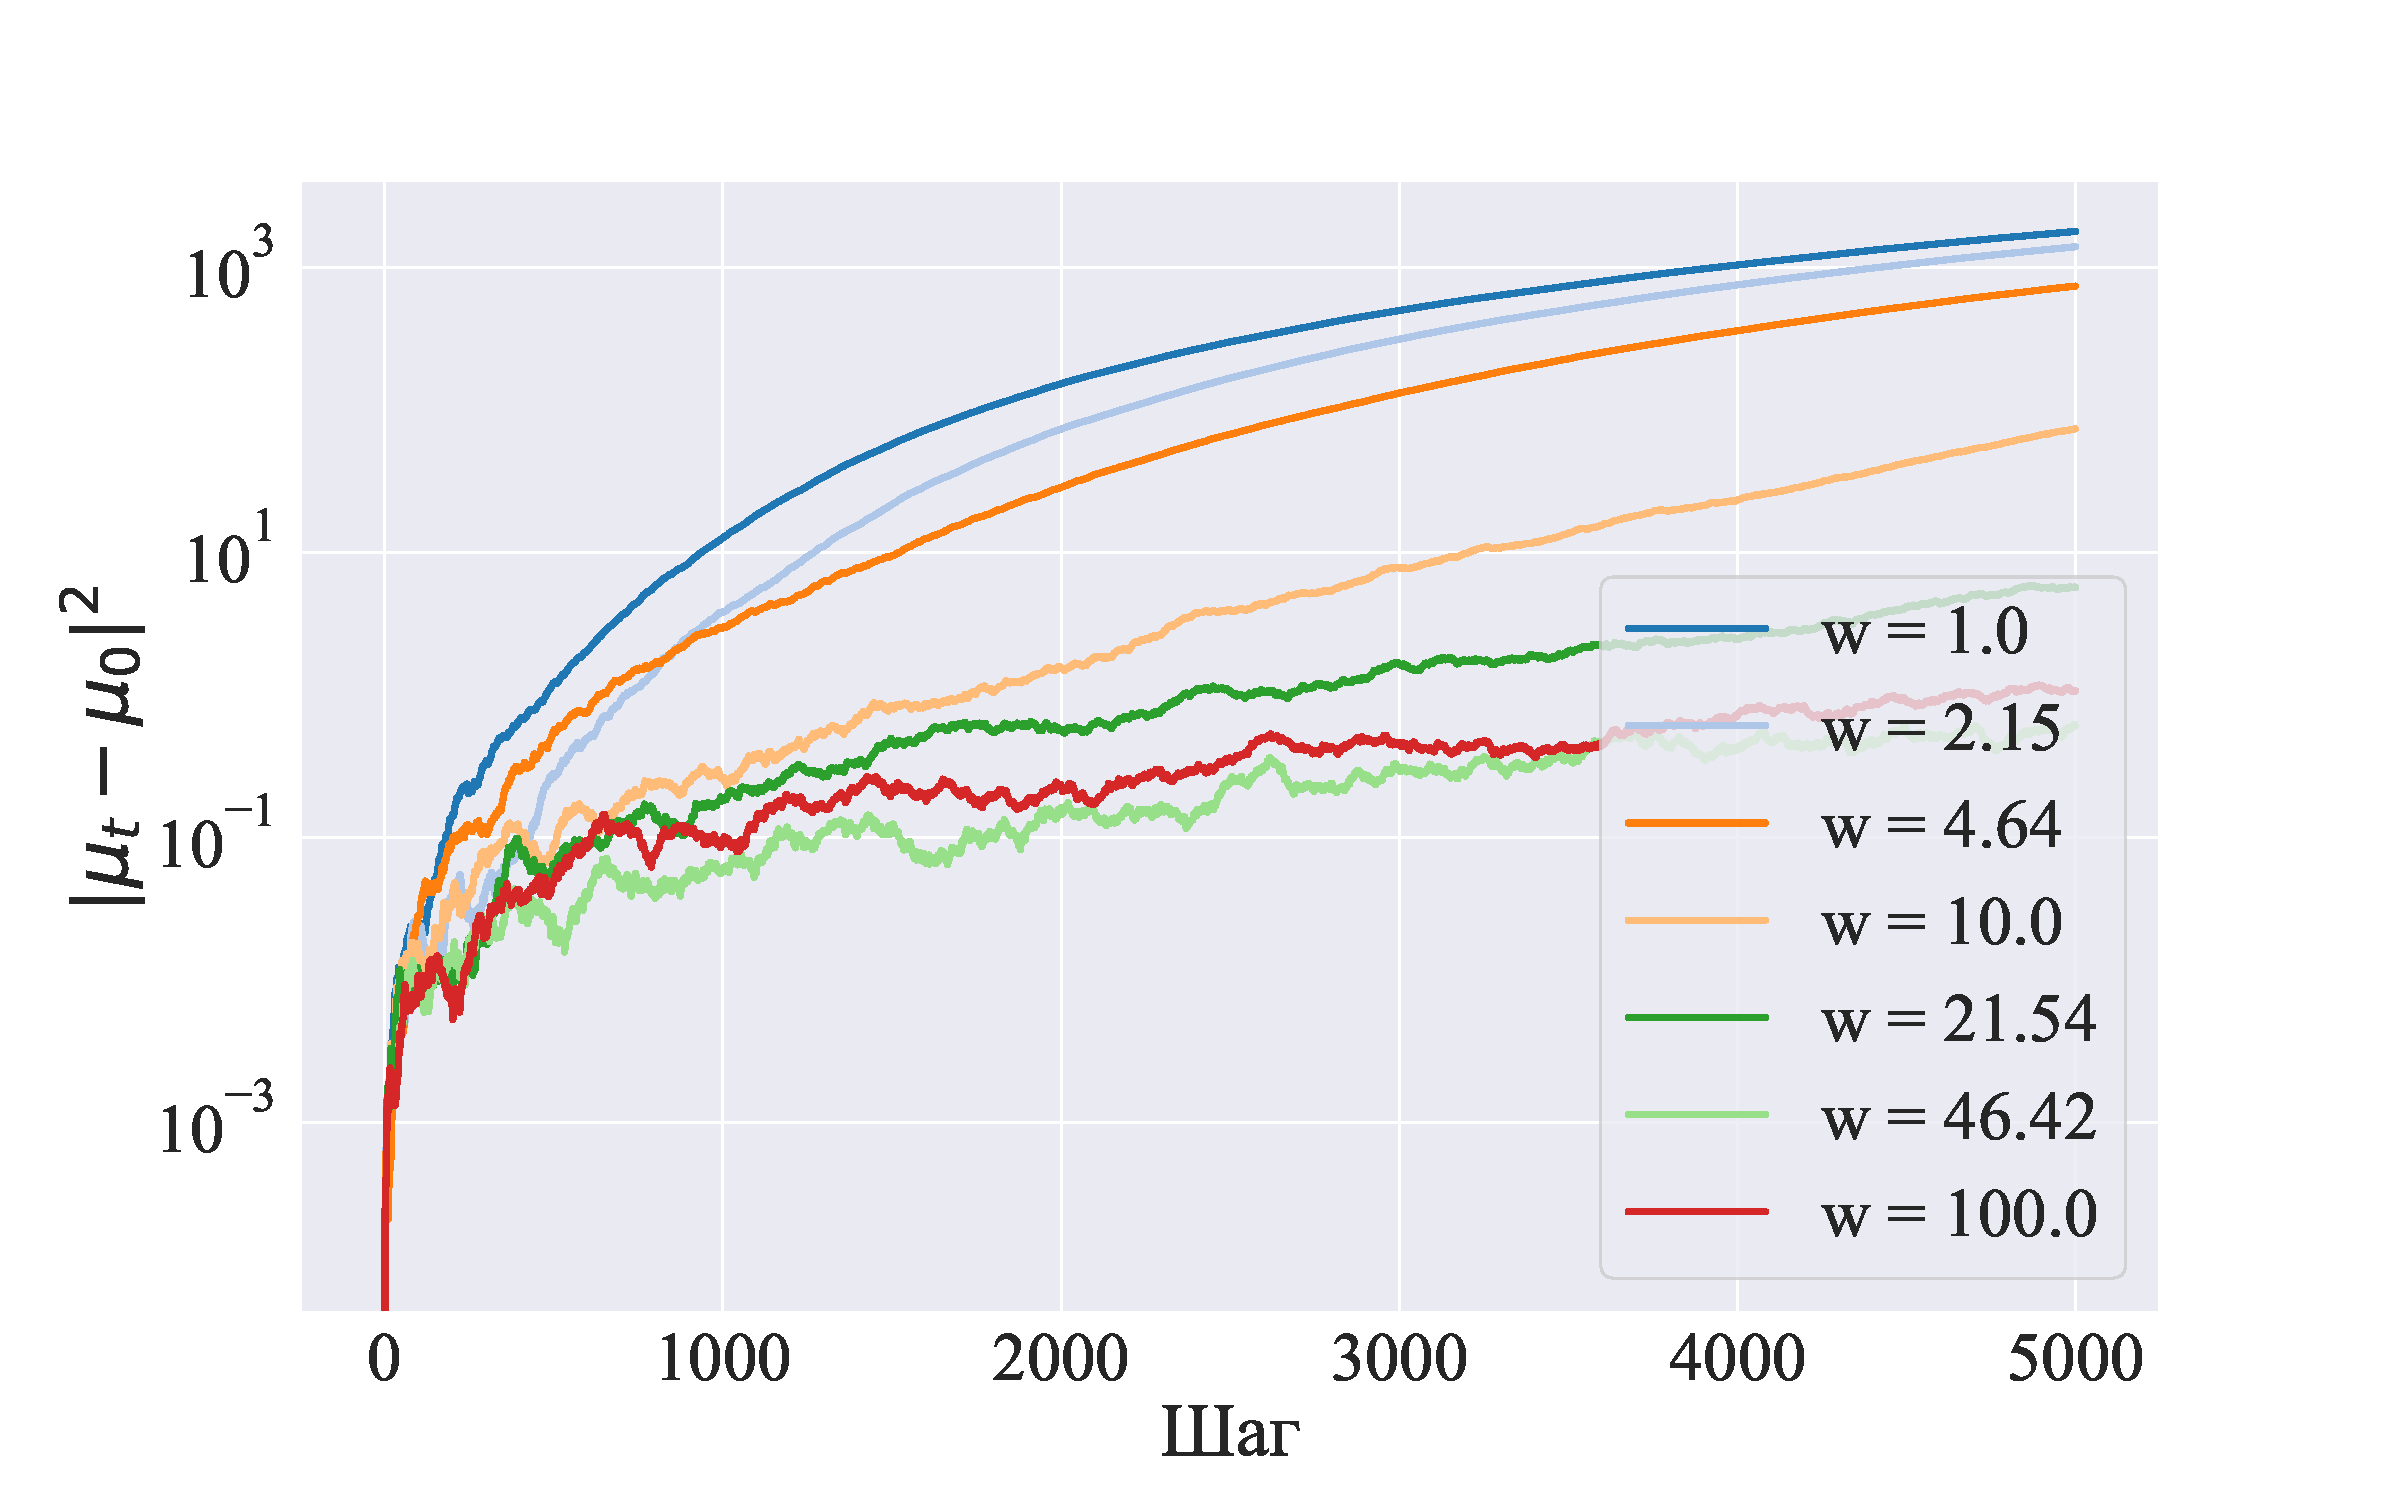
\includegraphics[width=0.5\textwidth]{../figures/norm_interest.pdf}
    \hfill
    \caption{Логарифм нормы интереса на очередном шаге рекомендации.}
    \label{fig1}
    \hfill
    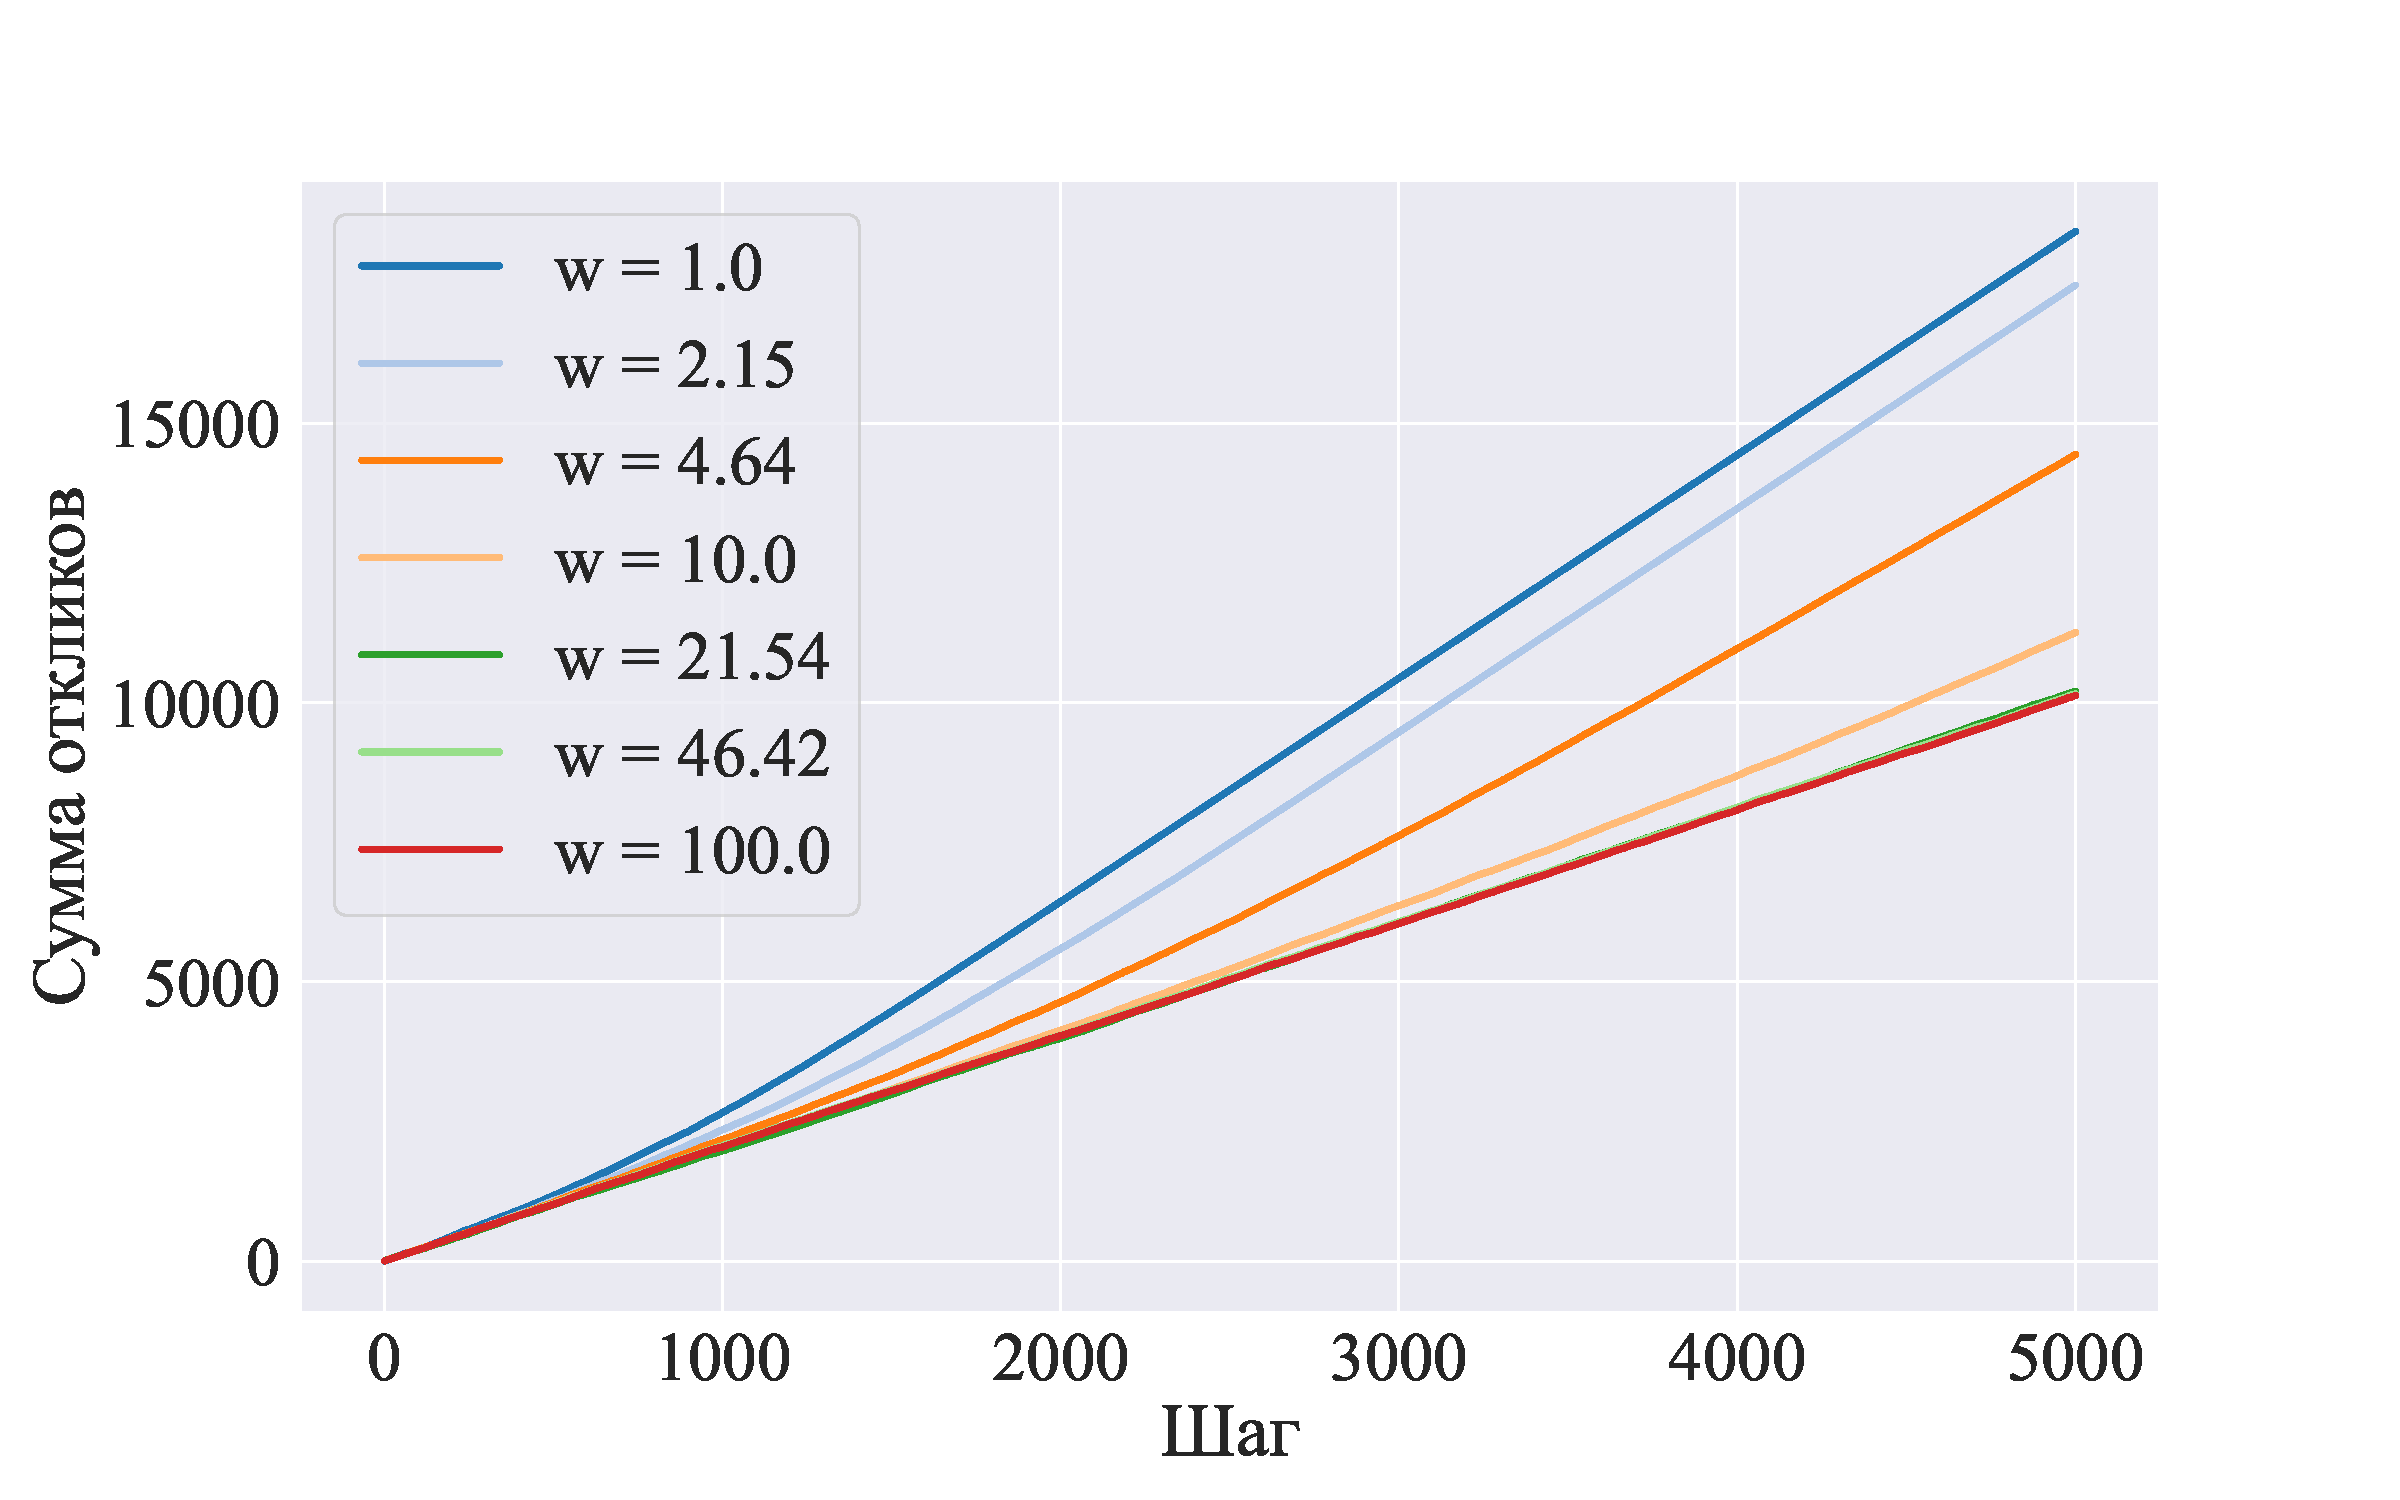
\includegraphics[width=0.5\textwidth]{../figures/rewards.pdf}
    \hfill
    \caption{Суммы наград на очередном шаге рекомендации.}
    \label{fig2}
  \end{multicols}
\end{figure}

На рис.$~\ref{fig3}$ изображён разброс значений нормы интереса для 30 запусков эксперимента.
На рис.$~\ref{fig8},\ref{fig9}$ сравниваются рекомендательные системы с различными алгоритмами рекомендации: Thompson Sampling, Random, Epsilon Greedy, Optimal.

В случае аддитивного шума для всех моделей тоже наблюдается образование петли (см. рис.$~\ref{fig9}$). 
Только для случайной модели заметены существенные различия, но тренд неограниченного роста интереса всё равно присутствует.   


Для накопительного шума для всех моделей, кроме оптимальной, тоже наблюдается образование петли (см. рис.$~\ref{fig8}$). 

\begin{figure}[h]
  \begin{multicols}{2}
    \hfill
    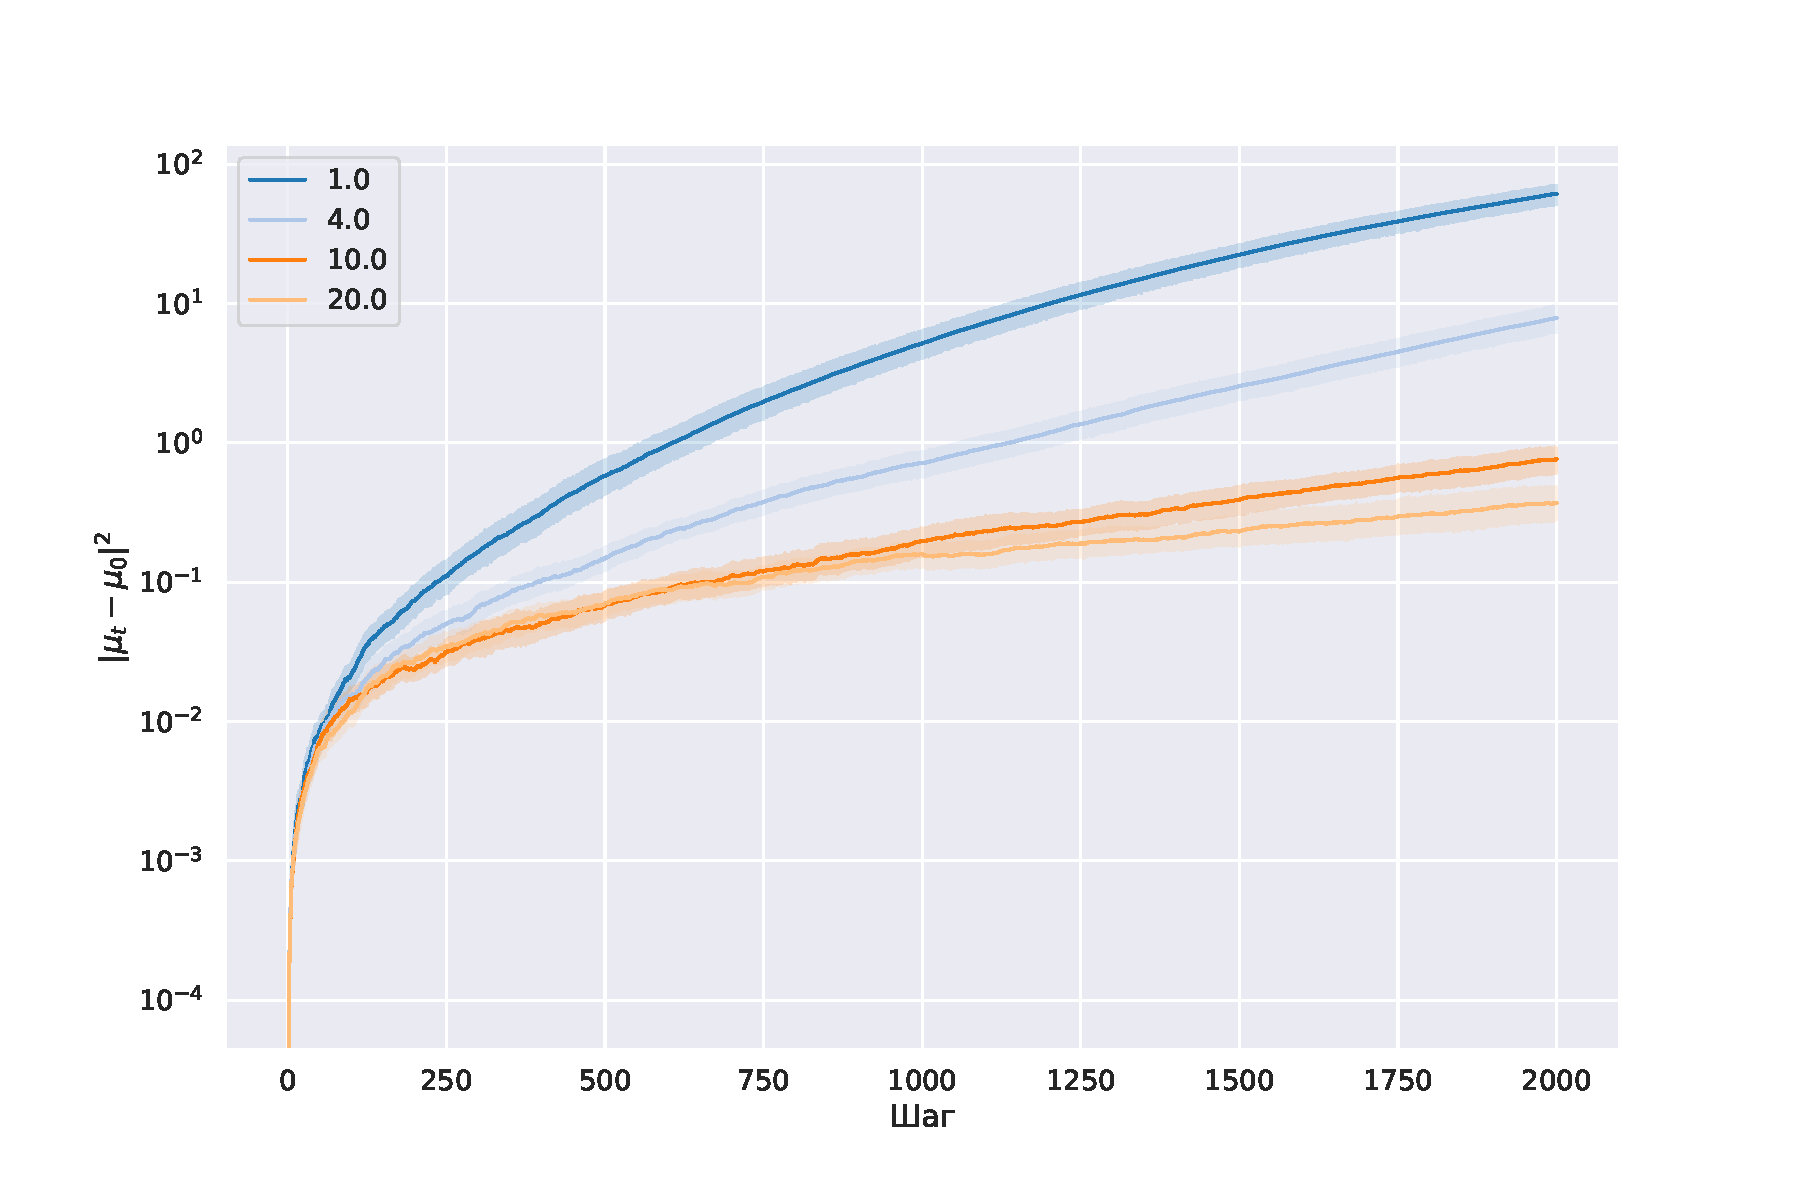
\includegraphics[width=0.5\textwidth]{../figures/var_norm_interest.pdf}
    \hfill
    \caption{Разброс логарифма нормы интереса от шага.}
    \label{fig3}
    \hfill
    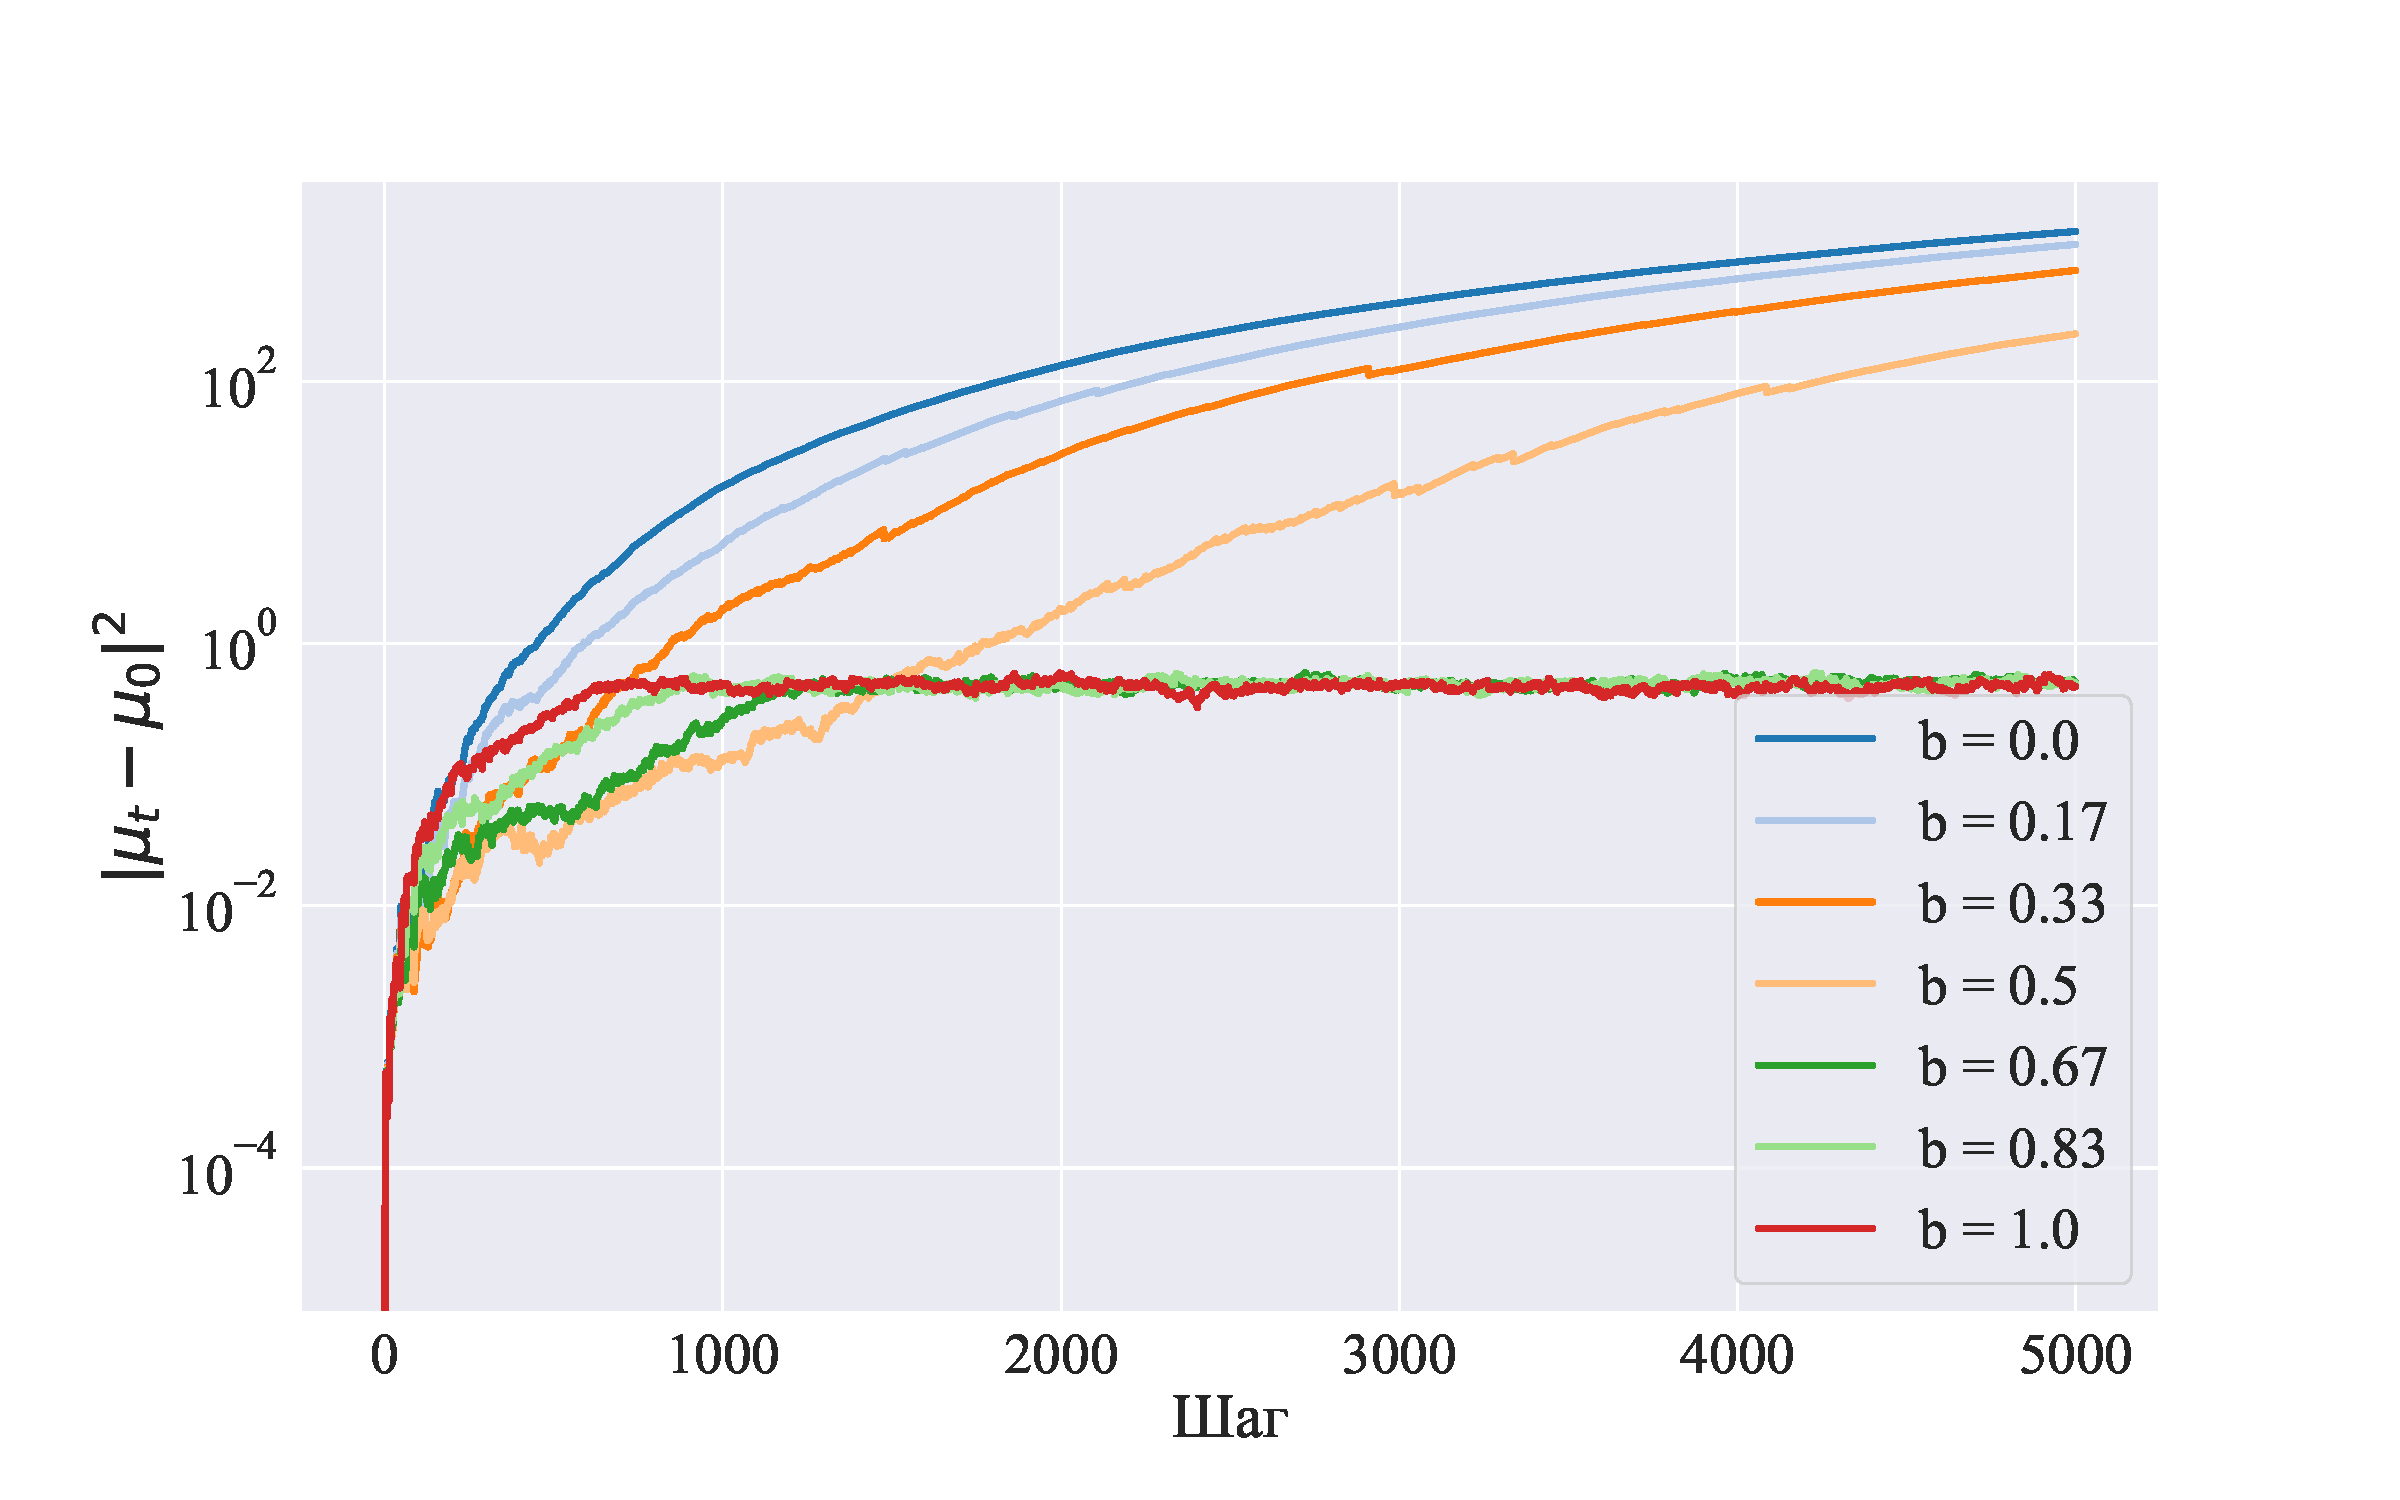
\includegraphics[width=0.5\textwidth]{../figures/winstreak_norm_interest.pdf}
    \caption{Зависимость нормы интереса от шага при различных параметров накопительного шума}
    \hfill
    \label{fig4}
  \end{multicols}
\end{figure}

\newpage

\begin{figure}[h]
  \begin{multicols}{2}
    \hfill
    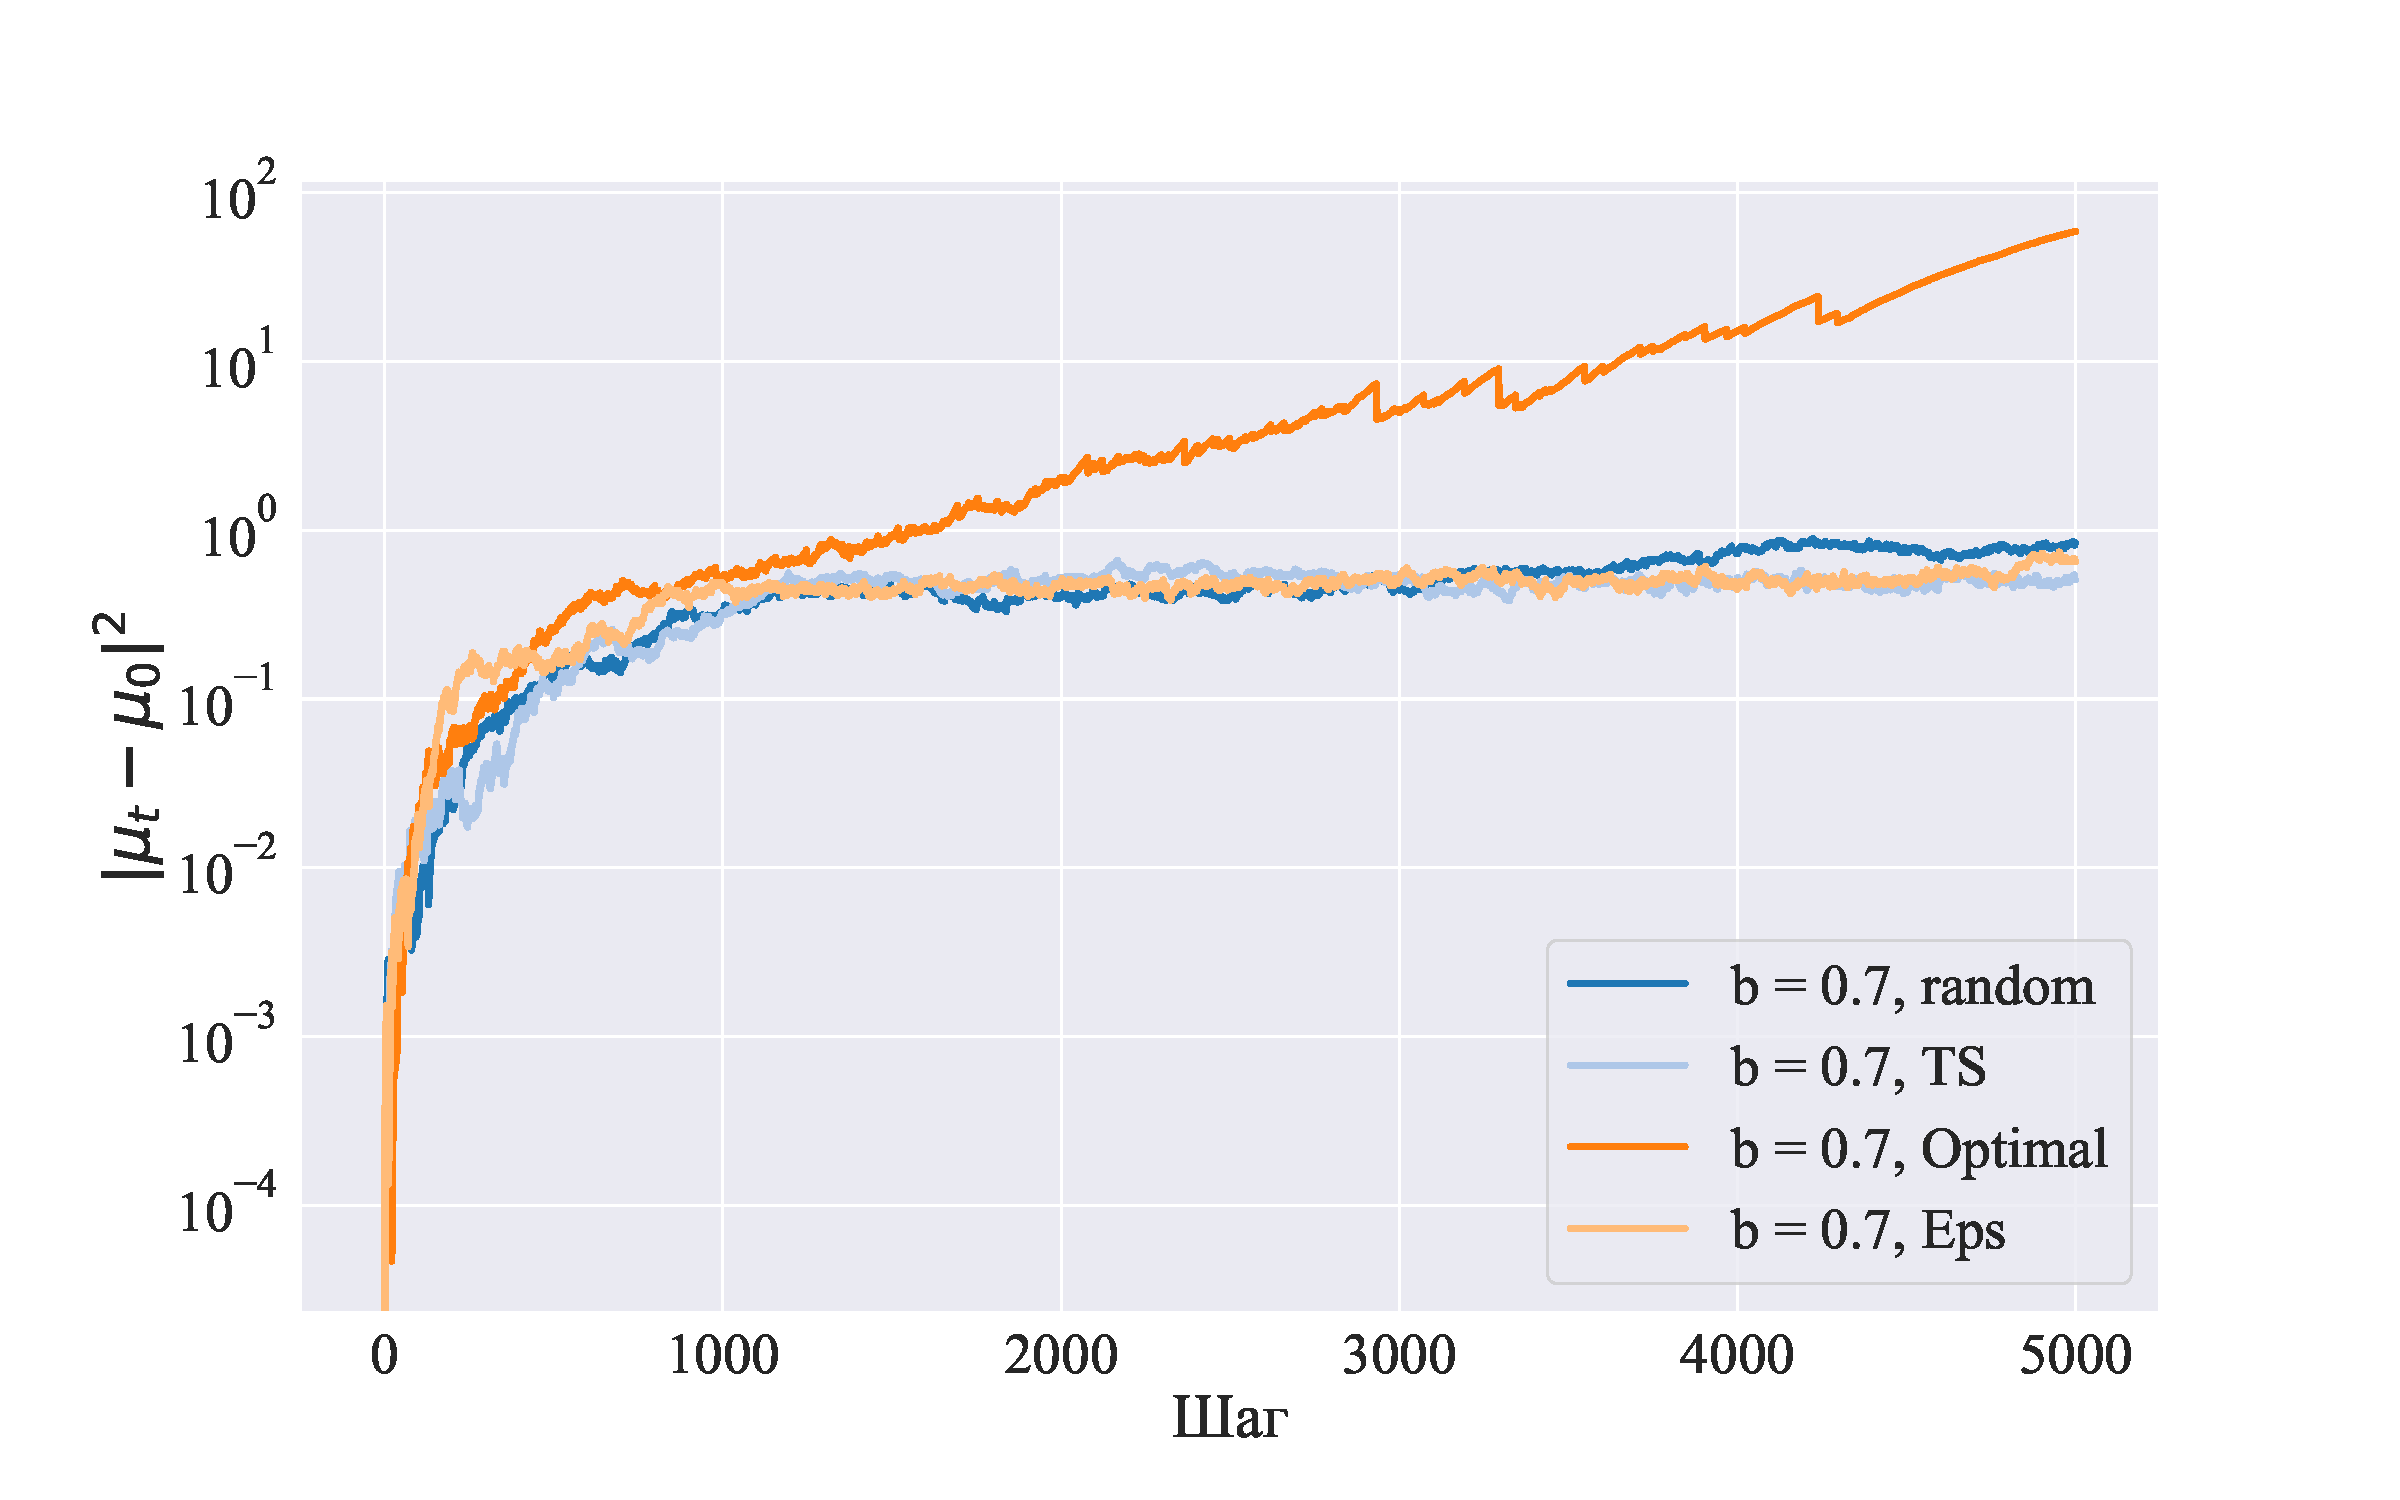
\includegraphics[width=0.5\textwidth]{../figures/compare_model_b.pdf}
    \hfill
    \caption{Сравнение различных алгоритмов рекомендации для накопительной модели шума}
    \label{fig8}
    \hfill
    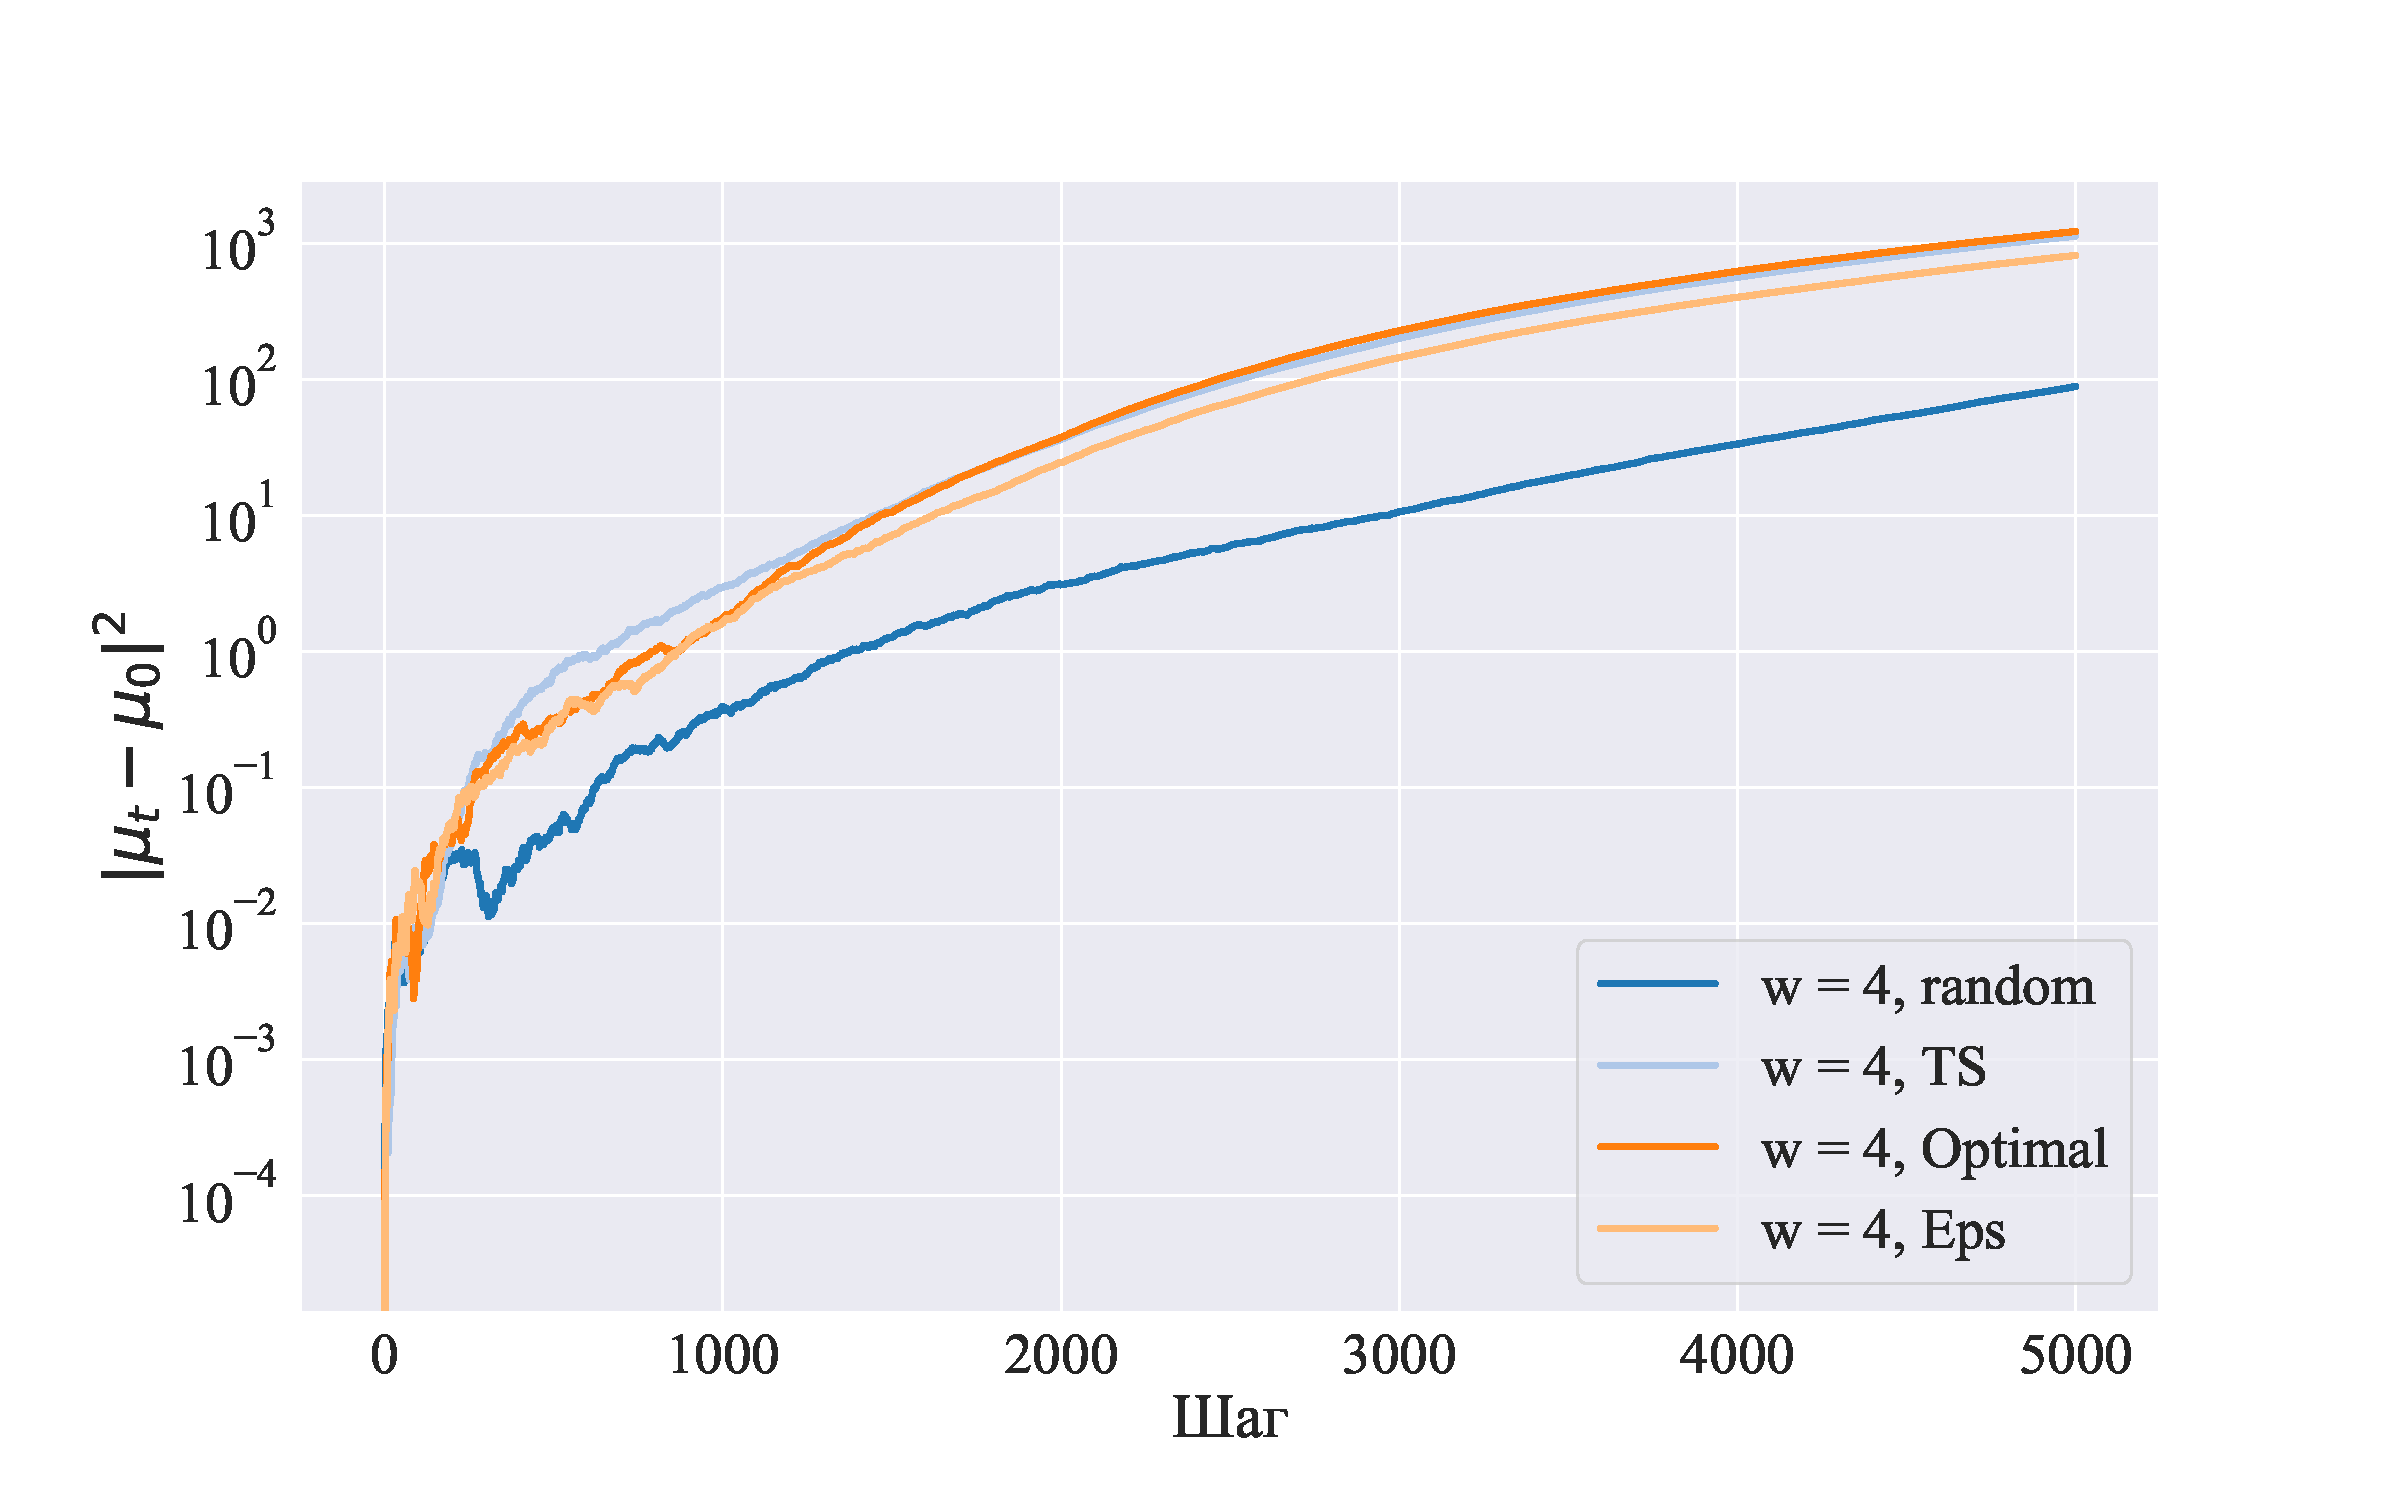
\includegraphics[width=0.5\textwidth]{../figures/compare_models_w.pdf}
    \hfill
    \caption{Сравнение различных алгоритмов рекомендации для аддитивной модели шума}
    \label{fig9}
  \end{multicols}
\end{figure}

\begin{figure}[h]
  \begin{multicols}{2}
    \hfill
    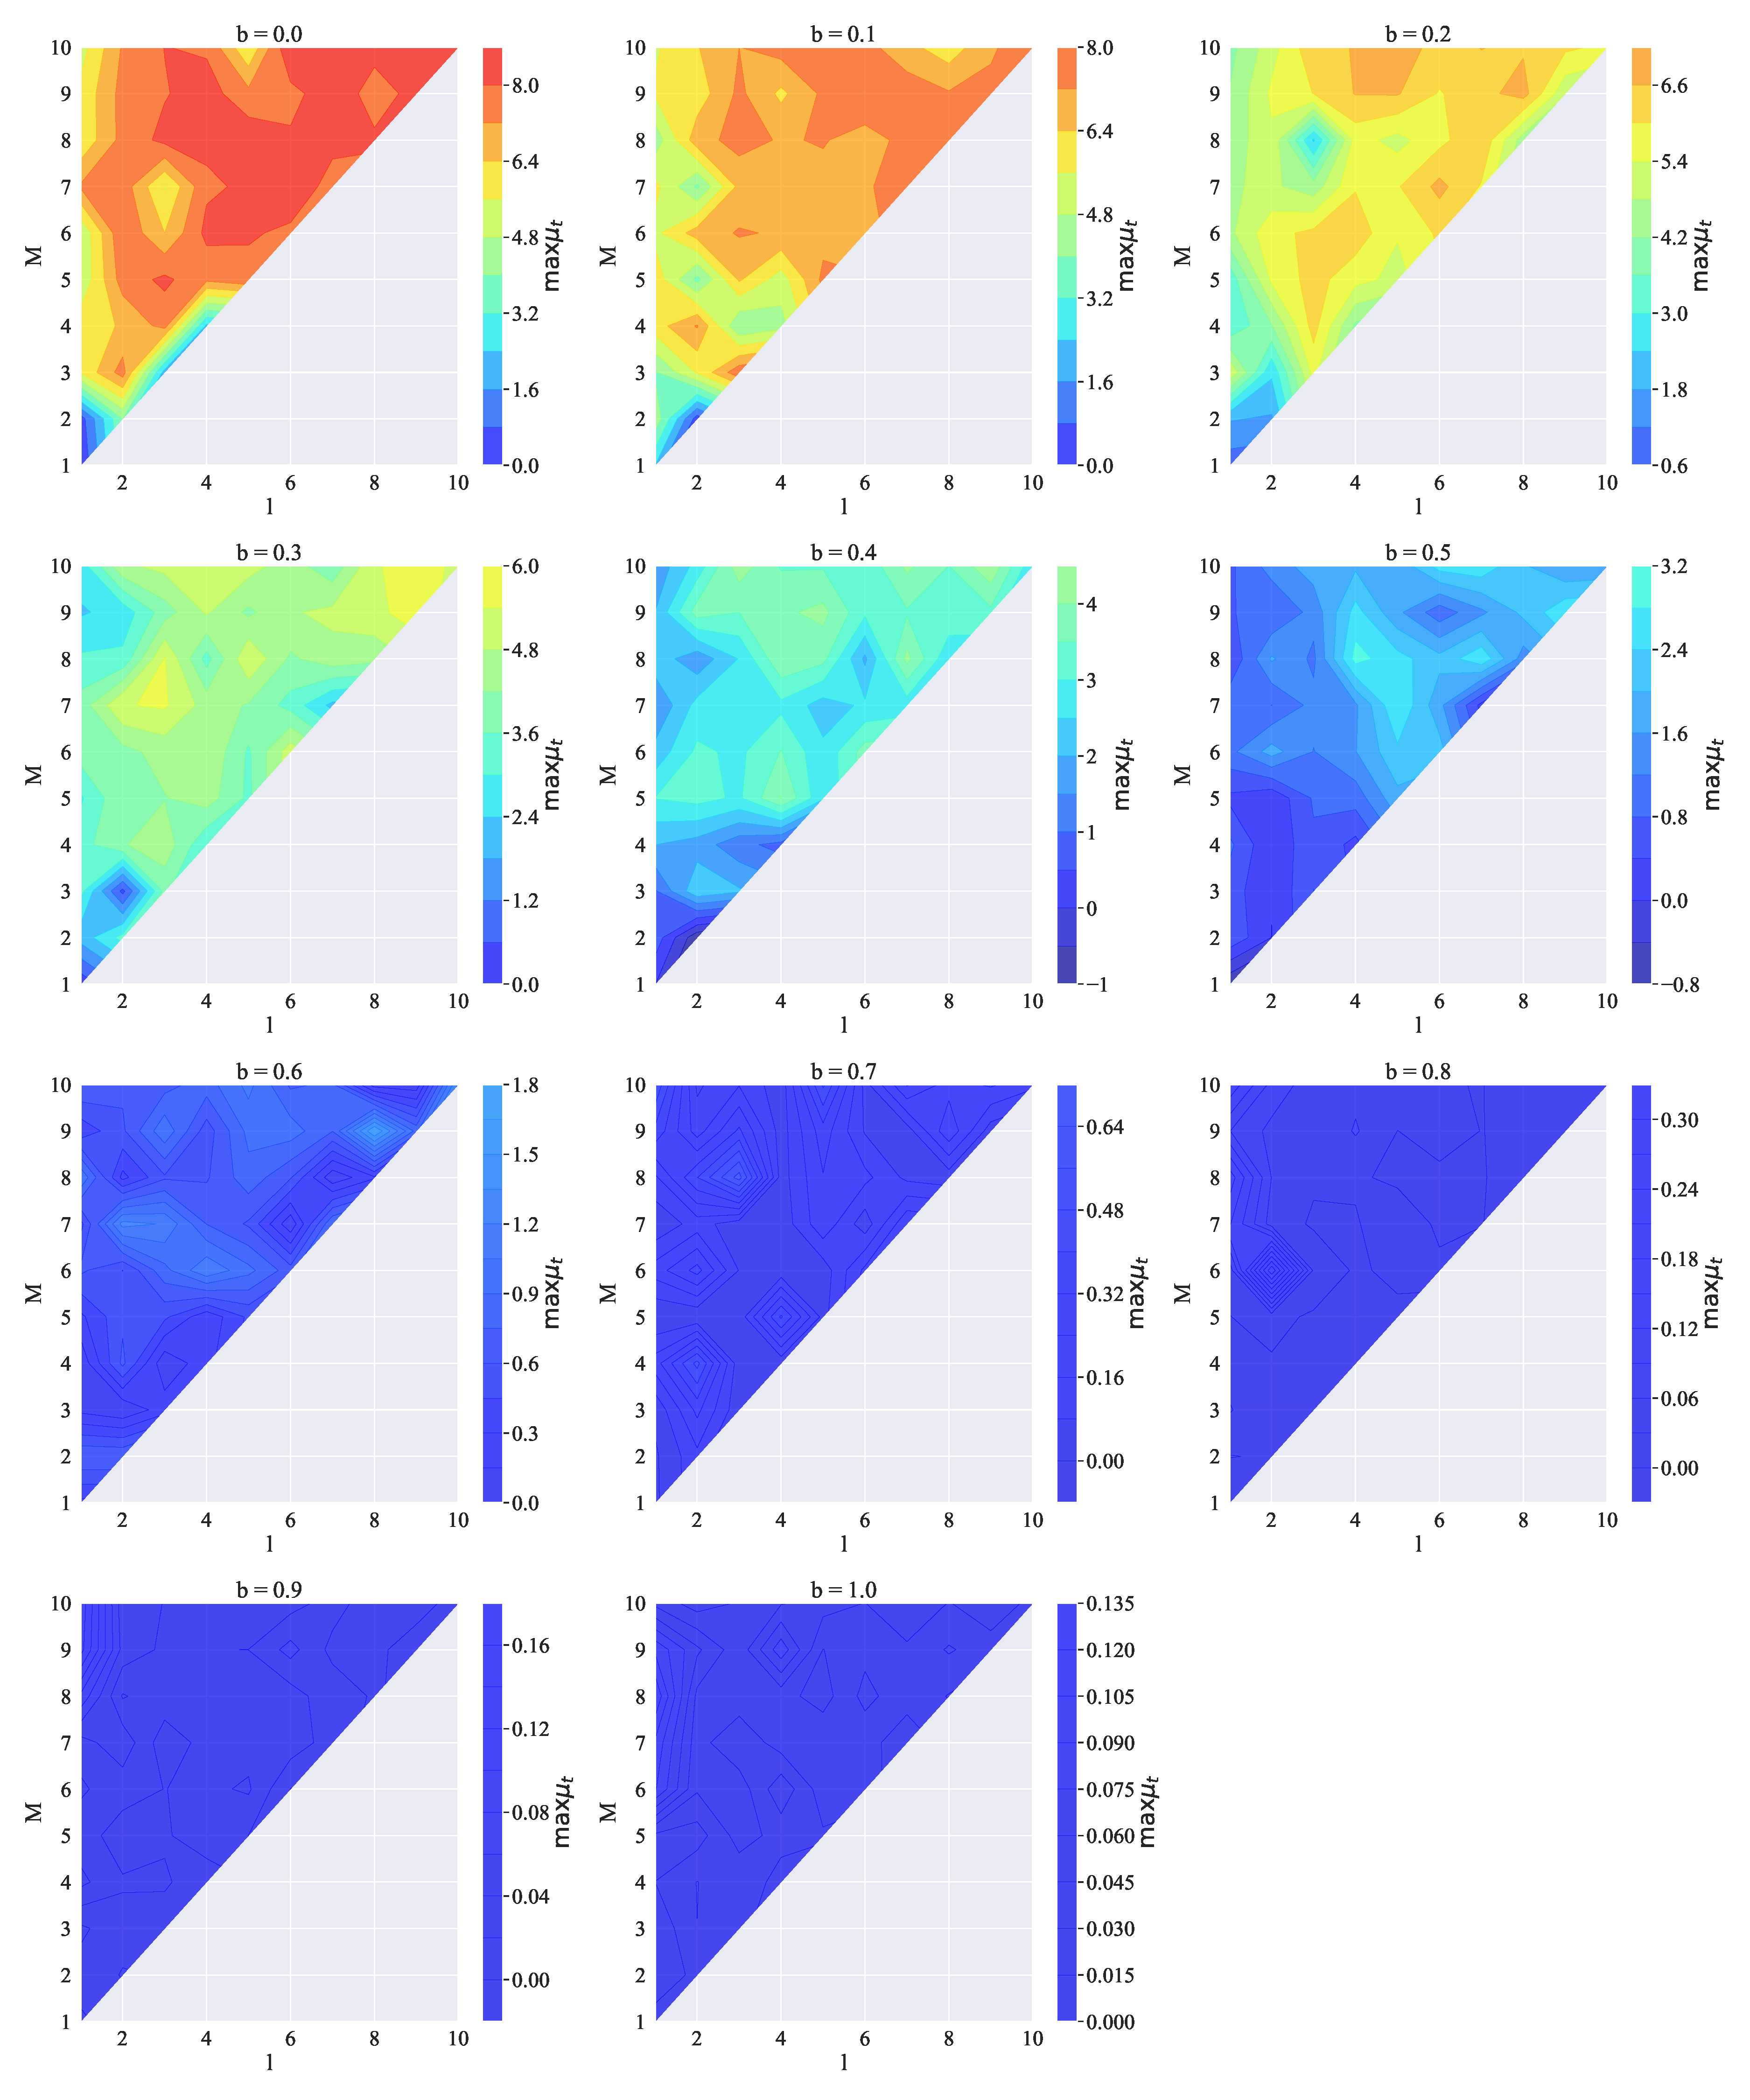
\includegraphics[width=0.5\textwidth]{../figures/countour_Mlb.pdf}
    \hfill
    \caption{Распределение максимумов значения интереса на шаге $T=2000$ для различных параметров модели и шума}
    \label{fig5}
    \hfill
    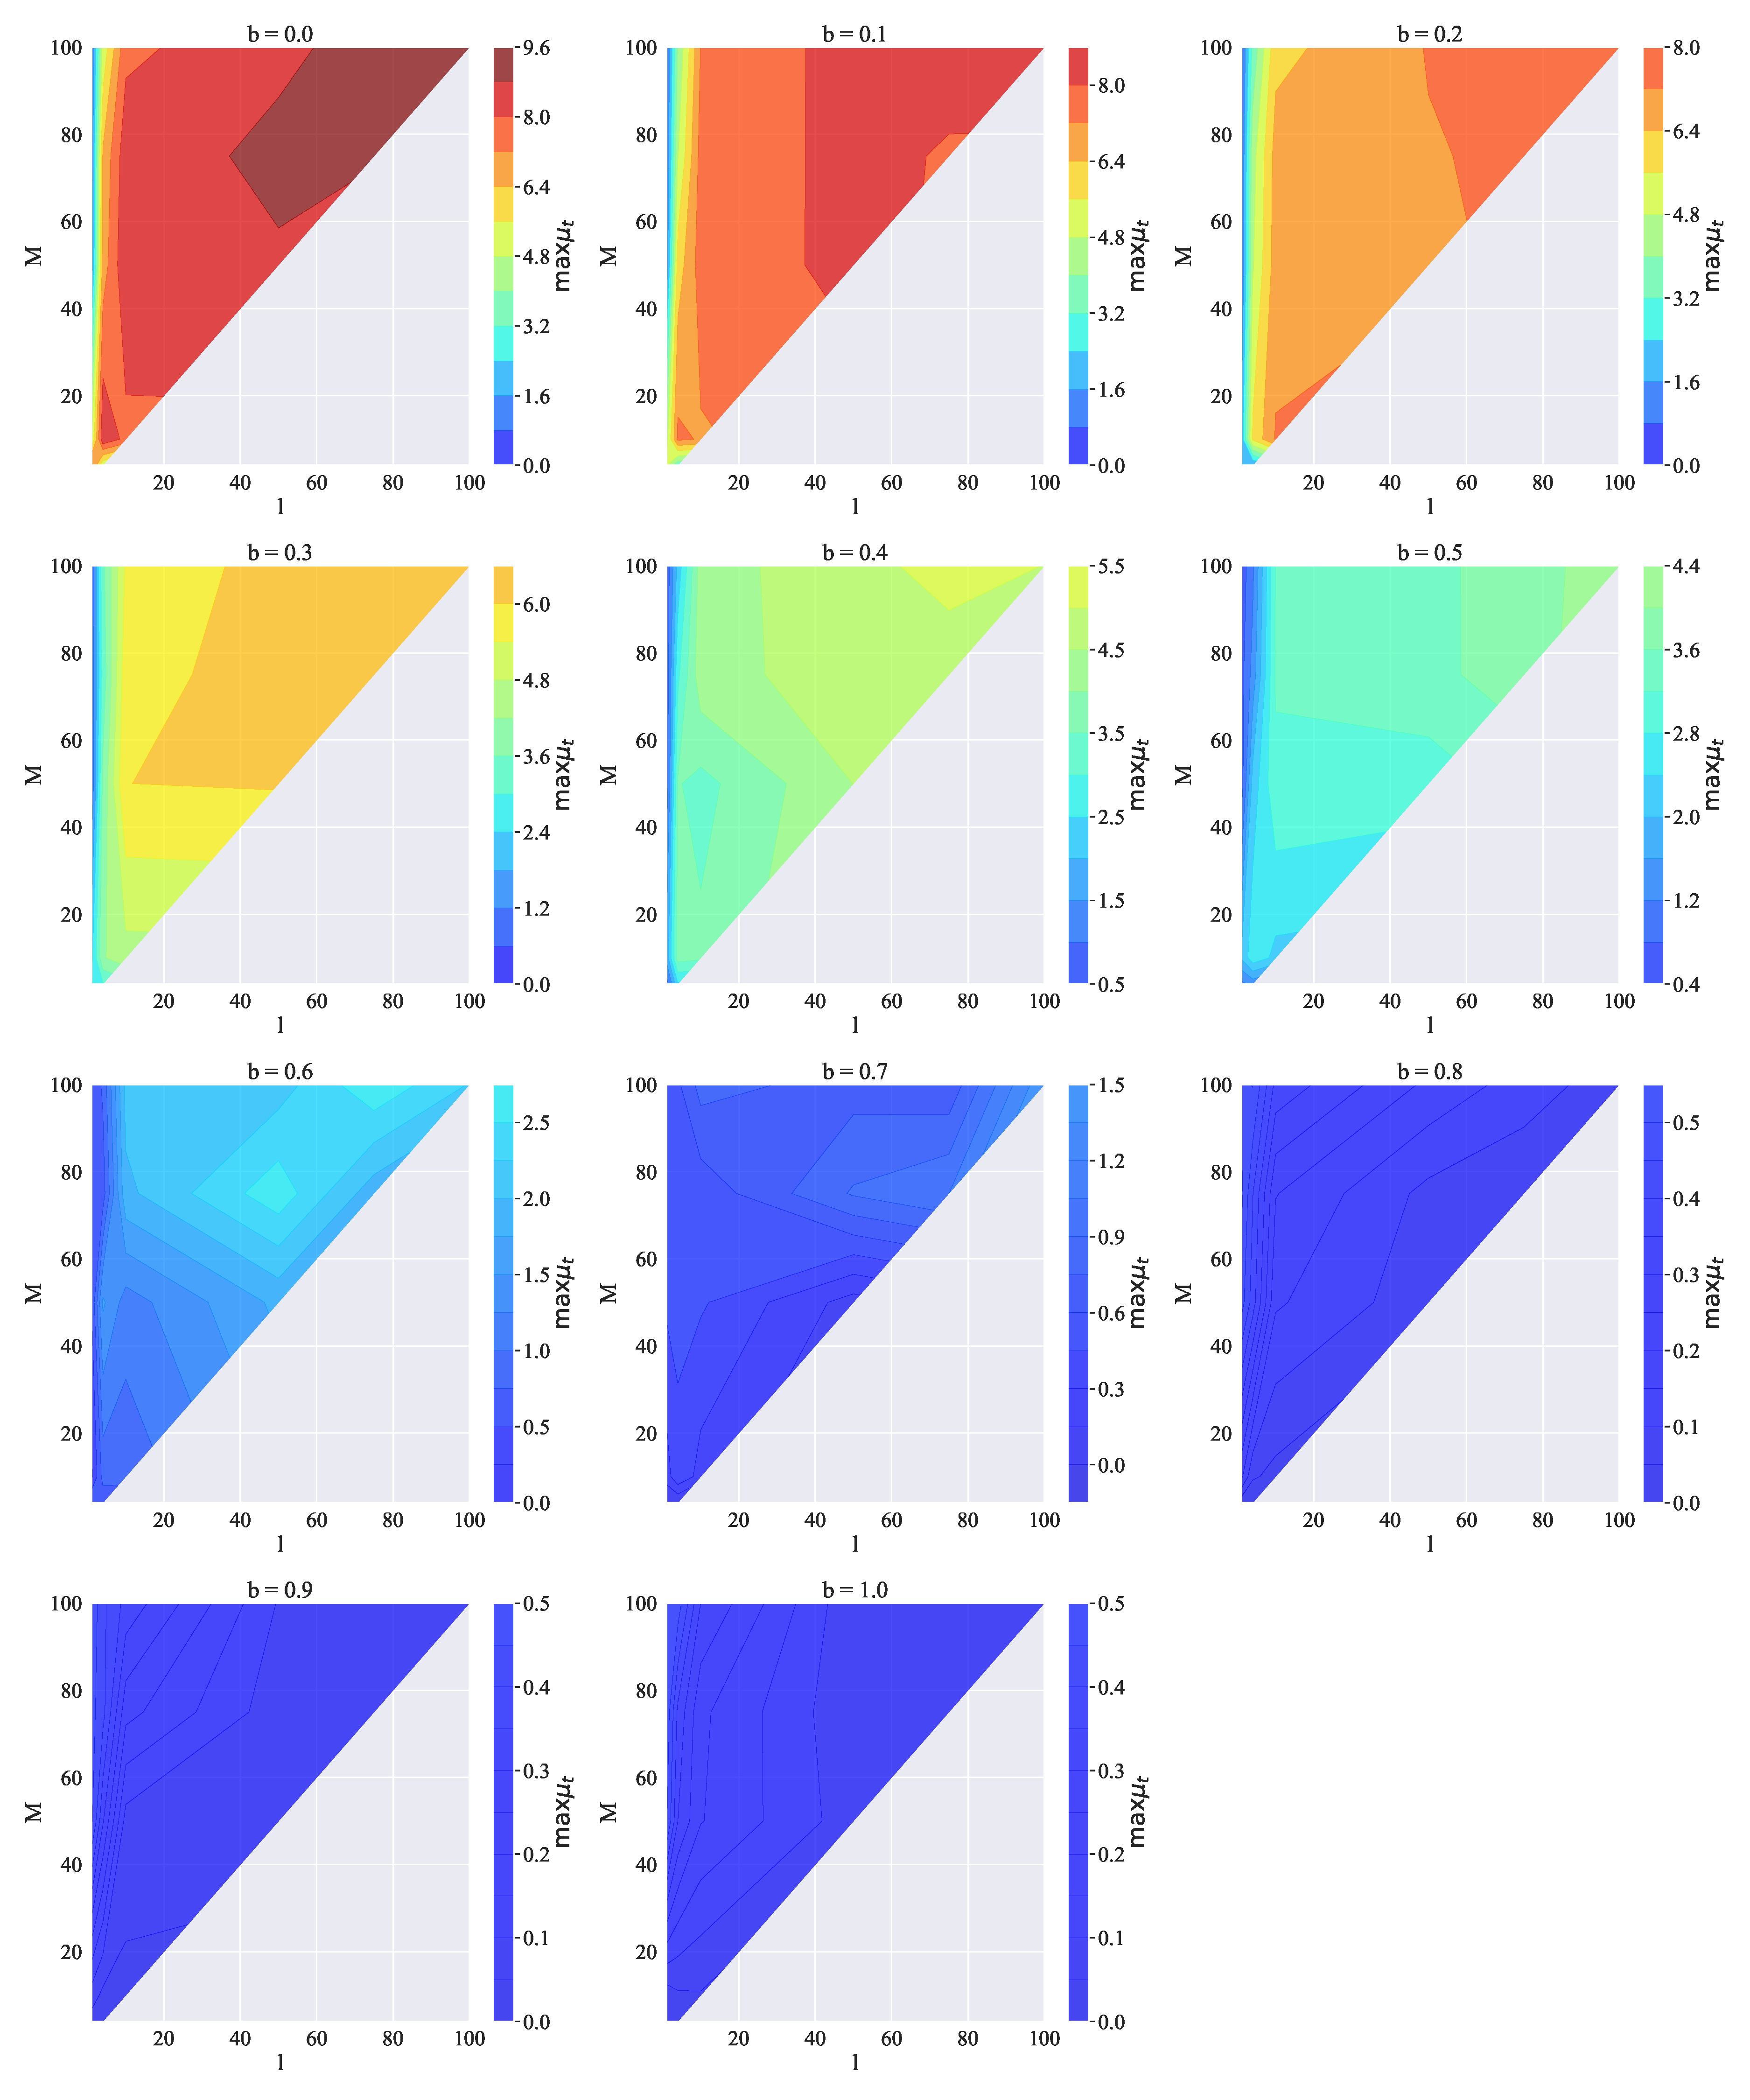
\includegraphics[width=0.5\textwidth]{../figures/countour_big_Mlb.pdf}
    \hfill
    \caption{Распределение максимумов значения интереса на шаге $T=2000$ для больших параметров модели}
    \label{fig6}
  \end{multicols}
\end{figure}
% На рис.$~\ref{fig4},~\ref{fig5}$ отоброженно влияние параметров шума на интерес. 
% Можно видеть, что увеличение шума замедляет рост интереса. 
% Это согласуется с полученным утверждением и рис$~\ref{fig1}$.

\newpage

\section{Заключение}
Поставлена задача существования петель скрытой обратной связи при наличии аддитвного шума в ответах пользователя и независимого обновления интереса.
Также был сформулирован накопительный шум, где присутсвует скоррелированность при обновлении интереса пользователя.
Для аддитвной модели шума было получено, что при любых параметрах возникают петли. 
Это также подверждается в эксперименте.
В случае накопительного шума на эксперименте было получено наличие порога, при котором петля отстутствует.

В дальнейшем требуется проверить гипотезу о возникновении петель при любом несмещённом аддитивном шума. 
Требуется получить теоретические обоснования отсутствия петли при накопительном шуме.
Также стоит расмотреть другие модели шума. 
%%%% если имеется doi цитируемого источника, необходимо его указать, см. пример в \bibitem{article}
%%%% DOI публикации, зарегистрированной в системе Crossref, можно получить по адресу http://www.crossref.org/guestquery/
\begin{thebibliography}{99}
\bibitem{webArticle}
    \BibAuthor{Ray~Jiang, Silvia~Chiappa, Tor~Lattimore,Andr{\'a}s Gy{\"o}rgy, Pushmeet~Kohli}
    Degenerate Feedback Loops in Recommender Systems//
    \BibJournal{CoRR}, 2019, Vol. abs/1902.10730,
	  URL: \BibUrl{https://arxiv.org/abs/1902.10730}.

\bibitem{Article}
    \BibAuthor{Khritankov, Anton}
    Hidden Feedback Loops in Machine Learning Systems: A simulation Model and Preliminary Results//
    \BibJournal{Springer}, 2021, P.~54--65.

\bibitem{webArticle}
    \BibAuthor{Daniel Russo, Benjamin Van Roy, Abbas Kazerouni, Ian Osband}
    A Tutorial on Thompson Sampling//
    \BibJournal{CoRR}, 2017, Vol. abs/1707.02038,
	  URL: \BibUrl{https://arxiv.org/abs/1707.02038}.

\bibitem{webArticle}
    \BibAuthor{Shipra Agrawal, Navin Goyal}
    Analysis of Thompson Sampling for the multi-armed//
    \BibJournal{CoRR}, 2011, Vol. abs/1111.1797,
	  URL: \BibUrl{https://arxiv.org/abs/1111.1797}.

\bibitem{Article}
    \BibAuthor{Giuseppe Burtini, Jason L. Loeppky, Ramon Lawrence}    
    Improving Online Marketing Experiments with Drifting Multi-armed Bandits//
    \BibJournal{SciTePress}, 2018, P.~630--636.

\bibitem{webArticle}
    \BibAuthor{David Krueger and Tegan Maharaj and Jan Leike}    
    Hidden Incentives for Auto-Induced Distributional Shift//
    \BibJournal{CoRR}, 2020, Vol. abs/2009.09153.

\bibitem{webArticle}
    \BibAuthor{Wilbert Samuel Rossi, Jan Willem Polderman, Paolo Frasca}    
    The closed loop between opinion formation and personalised recommendations//
    \BibJournal{CoRR}, 2018, Vol. abs/1809.04644.

\bibitem{Article}
    \BibAuthor{Pedreschi, D. and Miliou, I. and European Parliament. Directorate-General for Internal Policies of the Union}    
    Artificial Intelligence (AI): new developments and innovations applied to e-commerce//
    \BibJournal{European Parliament}, 2020.

\bibitem{Article}
    \BibAuthor{Dominic DiFranzo, Kristine Gloria-Garcia}    
    Filter bubbles and fake news//
    \BibJournal{XRDS}, 2017.

\bibitem{webArticle}
    \BibAuthor{Пилькевич Антон, Хританков Антон}    
    Условие существования петель скрытой обратной связи в рекомендательных системах с учётом шума//
    %\BibJournal{CoRR}, 2011, Vol. abs/1111.1797,
	  URL: \BibUrl{github.com/Intelligent-Systems-Phystech/2021-Project-74}.
\end{thebibliography}

\section{Приложение}\label{application}
\begin{statement}
  Пусть TS работает в особом режиме начиная с какого-то момента времени $\tau$. Тогда при $w \geq 0 : \lim_{t \to \infty} \|\mu_t - \mu_0 \|_2 = \infty.$
\end{statement}
$\textbf{Доказательство. }$ 
Так как алгоритм работает в особом режиме, то при $t \geq \tau$ извествно какие объекты он будет рекомендовать.
Для случая нормы интересов: 
\begin{gather*}
  \|\mu_t - \mu_0 \|^2_2 = \sum_{i=1}^M (\mu_t^i - \mu_0^i)^2,
\end{gather*}
с ростом $t$ ocновной вклад будут давать только $l < M$ объектов попавших в рекомендацию. 
Причём эти объекты известны и не меняются для очередного шага. 

Рассмотрим изменение интереса для произвольного $a \in M$. 
Обновление интереса происходит согласно: $\mu_t - \mu_{t-1} = \delta_t c_t - \delta (1 - c_t)$.
Случайные величины $\delta_t, c_t$ независимы, поэтому: \[\mathsf{E} \delta_t c_t = \mathsf{E} \delta_t \mathsf{E} c_t.\] 
Для удобства будем считать, что у нас $c_t \sim \text{Bern}_{\pm}(\sigma(\mu_t(a_t) + q_t))$
Тогда: 
\begin{gather*}
  \mathsf{E} (c_t |q_t = y) = 2 \sigma(\mathsf{E} \mu_{t-1} + y) - 1, \\
\end{gather*}

В случае $\mathsf{E}(\mathsf{E}(c_t|q_t)) > 0$ петля будет возникать, так как рост интереса в среднем положителен. 

Далее для простоты считается, что $\sigma(x) \approx \left(\frac{x}{4} + \frac{1}{2} \right) \cdot I[-2, 2] + I[2, \infty]$ и $p = 1$.
Задача в этом случае записывается так:
\begin{gather*}
  \mathsf{E} (c_t |q_t = y) \approx  2 \left(\frac{\mathsf{E} \mu_{t-1} + y}{4} + \frac{1}{2}\right) - 1.   
\end{gather*}
Теперь петля возникает при условии: $\mathsf{E}\sigma(x) > \frac{1}{2}$. 

Тогда остаётся посчитать:
\begin{gather*}
  \mathsf{E} \sigma(\mu_t) \approx \int_{-\infty}^{\infty} \left(\frac{\mathsf{E} \mu_t + y}{4} + \frac{1}{2} \right) I\{-2 < \mathsf{E}\mu_t +y < 2\} f(y)dy \\
  + \int_{-\infty}^{\infty} I\{2 < \mathsf{E}\mu_t +y \}f(y) dy = \\
  \int_{-2}^{2} \left(\frac{z}{4} + \frac{1}{2} \right) f_s(z)dz 
  + \int_{2}^{\infty} f_s(z) dz,
\end{gather*}
где $f_s(z)$ плотность $U[\mathsf{E}\mu_t - w, \mathsf{E}\mu_t + w]$.
Таким образом у нас возникает $6$ случаев.

\begin{enumerate}
  \item $\mathsf{E} \mu_t + w < -2$. Тогда, очевидно:
    \begin{gather*}
      \mathsf{E}\sigma(\mu_t) = 0 \to \mathsf{E}(\mathsf{E}(c_t|q_t)) = -1.
    \end{gather*}
    В этом случае интерес бесконечно убывает. 
    Так как рассмытривается норма интересов, то всё равно $(\mu_t -\mu_0)^2 \to \infty$ при $t\to\infty$. 

  \item $\mathsf{E}\mu_t - w < -2 < \mathsf{E}\mu_t + w < 2$. Тогда:
    \begin{gather*}
      \mathsf{E}\sigma(\mu_t) = \left. \frac{1}{16w} (y+2)^2 \right|_{-2}^{\mathsf{E}\mu_t + w} = 
        \frac{1}{16w} (\mathsf{E}\mu_t + w + 2)^2 < \frac{1}{2}, \\
        (\mathsf{E}\mu_t + w + 2)^2 < 8w, \\
    \begin{cases}
      \mathsf{E}\mu_t < -w - 2 + \sqrt{8w}, \\
      \mathsf{E}\mu_t > -w - 2 - \sqrt{8w}, 
    \end{cases} \to \text{рост}.
    \end{gather*}
    В случае $\mathsf{E}\sigma(\mu_t) > \frac{1}{2}$ система будет несовместна. 

  \item $\mathsf{E}\mu_t - w < -2, \mathsf{E}\mu_t + w > 2$. 
    \begin{gather*}
      \mathsf{E}\sigma(\mu_t) = \left. \frac{1}{16 w} (y+2)^2 \right|_{-2}^{2} + \frac{1}{2 w}(\mathsf{E}\mu_t + w -2) = \\
        \frac{1}{w} + \frac{\mathsf{E}\mu_t+w}{2w} - \frac{1}{w} = \frac{\mathsf{E}\mu_t + w}{2 w} > \frac{1}{2} \Rightarrow \\
        \mathsf{E}\mu_t > 0, w > 2 \to \text{ рост}.
    \end{gather*}
  
  \item $\mathsf{E}\mu_t - w > -2, \mathsf{E}\mu_t + w < 2$. Тогда:
    \begin{gather*}
      \mathsf{E}\sigma(\mu_t) = \left. \frac{1}{16 w} (y+2)^2 \right|_{\mathsf{E}\mu_t - w}^{\mathsf{E}\mu_t + w} > \frac{1}{2},\\
        (\mathsf{E}\mu_t + w + 2)^2 - (\mathsf{E}\mu_t - w + 2)^2 > 8w,\\
        (2 \mathsf{E}\mu_t + 4) \cdot 2w > 8w,\\
        \mathsf{E} \mu_t  > 0 \to \text{рост}. 
    \end{gather*}
  
  \item $\mathsf{E}\mu_t - w > -2, \mathsf{E}\mu_t + w > 2$. Тогда: 
    \begin{gather*}
      \mathsf{E}\sigma(\mu_t) = \left. \frac{1}{16 w} (y+2)^2 \right|_{\mathsf{E}\mu_t-w}^{2} + \left. \frac{1}{2w}\right|_{2}^{\mathsf{E}\mu_t + w} = \\ 
          \frac{1}{16 w} \left( 16 - (\mathsf{E} \mu_t-w+2)^2 \right) + \frac{1}{2 w}(\mathsf{E}\mu_t + w -2) = \\
          \frac{1}{w} - \frac{(\mathsf{E}\mu_t-w+2)^2}{16w} + \frac{\mathsf{E}\mu_t+w}{2w} - \frac{1}{w} = \\
          -\frac{1}{16w} (\mathsf{E}^2\mu_t - 2(w-2)\mathsf{E}\mu_t + (w-2)^2) + \frac{\mathsf{E}\mu_t + w}{2 w} > \frac{1}{2} \Rightarrow \\
          \mathsf{E}^2\mu_t - 2(w-2)\mathsf{E}\mu_t + (w-2)^2 - 8(\mathsf{E}\mu + w) + 8w < 0, \\
          \mathsf{E}^2\mu_t - 2(w+2)\mathsf{E}\mu_t + (w-2)^2 < 0, \\
          \left(\mathsf{E}\mu_t - (w+2) \right)^2 - (w+2)^2 + (w-2)^2 < 0, \\
          (\mathsf{E}\mu_t - (w+2))^2 - 8w < 0, \\
    \begin{cases}
      \mathsf{E}\mu_t < w + 2 + \sqrt{8w}, \\
      \mathsf{E}\mu_t > w + 2 - \sqrt{8w}, \\
    \end{cases} \to \text{рост}.
    \end{gather*}
  
  \item $\mathsf{E}\mu_t - w > 2$. Тогда: 
    \begin{gather*}
      \mathsf{E}\sigma(\mu_t) = 1 > \frac{1}{2}.
    \end{gather*}
\end{enumerate}

Во всех случаях при заданных условиях удалось отделить от нуля изменение интереса: 
\[
  \mathsf{E}(\mu_{t} - \mu_{t-1}) = \mathsf{E}\delta_t \cdot \mathsf{E}(\mathsf{E}(c_t|q_t)) > 0.
\]
Поэтому существет $m > 0$ такое, что 
\[
  \mathsf{E}(\mu_{t} - \mu_{t-1}) = \mathsf{E}\delta_t \cdot \mathsf{E}(\mathsf{E}(c_t|q_t)) > m > 0.
\]
Тогда 
\[\mathsf{E}^2(\mu_{t} - \mu_{0}) > t^2 \cdot m^2 \to \infty \text{ при } t \to \infty.\]
Раз одно слагомое стремится к бесконечности, то:
\[\mathsf{E}\|\mu_t - \mu_0 \|^2_2 \to \infty \text{ при } t \to \infty.\]

%%%% если имеется doi цитируемого источника, необходимо его указать, см. пример в \bibitem{article}
%%%% DOI публикации, зарегистрированной в системе Crossref, можно получить по адресу http://www.crossref.org/guestquery/.

\end{document}
